\documentclass[krantz1]{krantz} %See documentation for other class options
\usepackage{fixltx2e,fix-cm}
\usepackage{amssymb}
\usepackage{amsmath}
\usepackage{graphicx}
\usepackage{subfigure}
\usepackage{makeidx}
\usepackage{multicol}
\usepackage{listings}
\usepackage{bbm}
\usepackage[skins]{tcolorbox}
\usepackage{enumitem}
%\usepackage[dvips]{hyperref}

%%%%%%%%%%%%%%%%%%%%%%%%%%%%%%%%%%
\usepackage{listings}
\usepackage{xcolor}

\definecolor{codegreen}{rgb}{0,0.6,0}
\definecolor{codegray}{rgb}{0.5,0.5,0.5}
\definecolor{codepurple}{rgb}{0.58,0,0.82}
\definecolor{backcolour}{rgb}{0.95,0.95,0.92}

\lstdefinestyle{mystyle}{
	backgroundcolor=\color{backcolour},   
	commentstyle=\color{codegreen},
	keywordstyle=\color{magenta},
	numberstyle=\tiny\color{codegray},
	stringstyle=\color{codepurple},
	basicstyle=\ttfamily\footnotesize,
	breakatwhitespace=false,         
	breaklines=true,    captionpos=b,                    
	keepspaces=true, numbers=left,                    
	numbersep=5pt, showspaces=false,                
	showstringspaces=false, showtabs=false, tabsize=2}
\lstset{style=mystyle}
%%%%%%%%%%%%%%%%%%%%%%%%%%%%%%%%%%%%%%%%%%%%%


\makeindex

\usepackage{booktabs}
 %place custom commands and macros here

\begin{document}

\frontmatter

\title{Krantz Template} %This is a placeholder titlepage, it will not be final.
\author{Yours Truly}
%%%\maketitle

%%%Placeholder for front matter

\halftitle{\Large{\noindent Solution Manual\\
		Introduction to Bayesian Inference:\\
		A GUIded tour using R}}


\booktitle{\Large{\noindent Solution Manual\\
		Introduction to Bayesian Inference:\\
		A GUIded tour using R\\
		
		by Andrés Ramírez-Hassan, PhD. Statistical Science.}}

% \locpage

\cleardoublepage
\thispagestyle{empty}
\vspace*{\stretch{1}}
\begin{center}
\Large\itshape
To my parents, Nancy and Orlando.
\end{center}
\vspace{\stretch{2}}
\cleardoublepage
\setcounter{page}{7} %previous pages will be reserved for frontmatter to be added in later.
\tableofcontents
\chapter*{Foreword}
I am delighted to introduce the first book on Multimedia Data Mining.  When I came to know about this book project undertaken by two of the most active young researchers in the field, I was pleased that this book is coming in early stage of a field that will need it more than most fields do.  In most emerging research fields, a book can play a significant role in bringing some maturity to the field.  Research fields advance through research papers.  In research papers, however, only a limited perspective could be provided about the field, its application potential, and the techniques required and already developed in the field.  A book gives such a chance.  I liked the idea that there will be a book that will try to unify the field by bringing in disparate topics already available in several papers that are not easy to find and understand.  I was supportive of this book project even before I had seen any material on it.  The project was a brilliant and a bold idea by two active researchers.  Now that I have it on my screen, it appears to be even a better idea.  

Multimedia started gaining recognition in 1990s as a field.  Processing, storage, communication, and capture and display technologies had advanced enough that researchers and technologists started building approaches to combine information in multiple types of signals such as audio, images, video, and  text.  Multimedia computing and communication techniques recognize correlated information in multiple sources as well as insufficiency of information in any individual source.    By properly selecting sources to provide complementary information, such systems aspire, much like human perception system, to create a holistic picture of a situation using only partial information from separate sources.

Data mining is a direct outgrowth of progress in data storage and processing speeds.  When it became possible to store large volume of data and run different statistical computations to explore all possible and even unlikely correlations among data, the field of data mining was born.  Data mining allowed people to hypothesize relationships among data entities and explore support for those.  This field has been put to applications in many diverse domains and keeps getting more applications.  In fact many new fields are direct outgrowth of data mining and it is likely to become a powerful computational tool.\vadjust{\vfill\pagebreak}



\chapter*{Preface}
The main goal of this book is to make the Bayesian inferential framework more approachable to students, researchers, and practitioners who wish to understand and apply this statistical/econometric approach but do not have the time to develop programming skills. I have aimed to strike a balance between applicability and theory. This book provides a very user-friendly graphical user interface (GUI) to implement the most common regression models, while also covering the basic mathematical developments and their code implementation for those interested in advancing to more complex models.

\textbf{To instructors and students}

This book is divided into three parts: foundations (chapters 1 to 4), regression analysis (chapters 5 to 10), and \textit{Advanced} methods (chapters 11 to 14). Our graphical user interface (GUI) is designed for the second part. The source code can be found at \textbf{https://github.com/besmarter/BSTApp}. Instructors and students can access all the code, along with simulated and real datasets. There are three ways to install our GUI:

\begin{enumerate}
	\item Type \textbf{shiny::runGitHub(``besmarter/BSTApp", launch.browser=T)} in the \textbf{R} console or any \textbf{R} code editor and execute it.
	\item Visit \textbf{https://posit.cloud/content/4328505}, log in or sign up for \textbf{Posit Cloud}, navigate to the \textbf{BSTApp-master} folder in the \textbf{Files} tab of the right-bottom window, then click on the \textbf{app.R} file and select \textbf{Run App}.
	\item Use a \textbf{Docker} image by typing in the \textbf{Command Prompt}
	\begin{enumerate}
		\item docker pull magralo95/besmartergui:latest
		\item docker run --rm -p 3838:3838 magralo95/besmartergui
	\end{enumerate}
	Then users can access our GUI going to \textbf{http://localhost:3838/}. See Chapter \ref{chapGUI} for details.
\end{enumerate}

Students should have a basic understanding of probability theory and statistics, as well as some background in econometrics and time series, particularly regression analysis. Familiarity with standard univariate and multivariate probability distributions is strongly recommended. See a nice summary of useful probability distributions in \cite[p.~182-191]{greenberg2012introduction}. Additionally, students who wish to master the material in this book should have programming skills in \textbf{R} software.\footnote{An excellent starting point for \textbf{R} programming is the \textit{R Introduction Manual}: \textbf{https://cran.r-project.org/doc/manuals/r-release/R-intro.pdf}.}


I have included both formal and computational exercises at the end of each chapter to help students gain a better understanding of the material presented. A solutions manual for these exercises accompanies this book.

Instructors can use this book as a textbook for a course on introductory Bayesian Econometrics/Statistics, with a strong emphasis on implementation and applications. This book is intended to be complementary, rather than a substitute, for excellent resources on the topic, such as \cite{gelman2021bayesian}, \cite{chan2019bayesian}, \cite{rossi2012bayesian}, \cite{greenberg2012introduction}, \cite{geweke2005contemporary}, \cite{lancaster2004introduction}, and \cite{koop2003bayesian}.


\textbf{Acknowledgments}

I began developing our graphical user interface (GUI) in 2016, after being diagnosed with cervical dystonia. I worked on this side project during weekends, which I called ``nerd weekends,'' and it served as a form of release from my health condition. Once I began to recover, I invited Mateo Graciano, my former student, business partner, and friend, to join the project. He has been instrumental in developing our GUI, and I am enormously grateful to him. 

I would also like to thank the members of the BEsmarter research group at Universidad EAFIT, as well as the NUMBATs members at Monash University, for their valuable feedback and recommendations to improve our GUI.

This book is an extension of the paper \textit{A GUIded tour of Bayesian regression} \cite{Ramirez2020}, which serves as a brief user guide for our GUI. I decided to write this book to explain the underlying theory and code in our GUI, and to use it as a textbook in my course on Bayesian econometrics/statistics. I am grateful to my students in this course; their insights and thoughtful questions have deepened my understanding of the material.

I would like to thank Chris Parmeter for his valuable suggestions on how to present our user guide; Professors Raúl Pericchi and Juan Carlos Correa for introducing me to Bayesian statistics; and Liana Jacobi, Tomasz Wozniak, and Chun Fung Kwok (Jackson) from the University of Melbourne, as well as David Frazier from Monash University, for their engaging discussions and fruitful collaborations in Bayesian econometrics and statistics. I am also deeply grateful to Professor Peter Diggle for his unwavering support of my career, and especially to Professor Gael Martin, who gave me the opportunity to work with her and has been a constant source of intellectual inspiration.  

I also wish to acknowledge my colleagues and staff at Universidad EAFIT for their continuous support.  

Finally, I acknowledge the use of ChatGPT, which assisted me in improving the grammar, clarity, and flow of the text, as well as in tidying up the code presented in this book. Nevertheless, all concepts, mathematical developments, and underlying logic are entirely my own, based on my understanding and readings of the literature. Any remaining errors are solely my responsibility, for which I apologize in advance. I sincerely thank the reader and hope that this book proves useful.  

To my parents, Orlando and Nancy, who have always been there for me with their unconditional support. They have taught me that the primary aspect of human spiritual evolution is humility, a lesson I am still learning every day. To my fiancée, Estephania, for her unwavering love and support.





%%\listoffigures
%%\listoftables
%%%\twocolumn
\chapter*{Contributors}

\begin{multicols}{2}
\contributor{Michael Aftosmis}{NASA Ames Research Center}{Moffett Field, California}

\contributor{Pratul K. Agarwal}{Oak Ridge National Laboratory}{Oak Ridge, Tennessee}

\contributor{Sadaf R. Alam}{Oak Ridge National Laboratory}{Oak Ridge, Tennessee}

\contributor{Gabrielle Allen}{Louisiana State University}{Baton Rouge, Louisiana}

\contributor{Martin Sandve Aln{\ae}s}{Simula Research Laboratory and University of Oslo, Norway}{Norway}

\contributor{Steven F. Ashby} {Lawrence Livermore National Laboratory}{Livermore, California}

\contributor{David A. Bader} {Georgia Institute of Technology}{Atlanta, Georgia}

\contributor{Benjamin Bergen} {Los Alamos National Laboratory}{Los Alamos, New Mexico}

\contributor{Jonathan W. Berry} {Sandia National Laboratories}{Albuquerque, New Mexico}

\contributor{Martin Berzins}{University of Utah}{Salt Lake City, Utah}

\contributor{Abhinav Bhatele}{University of Illinois}{Urbana-Champaign, Illinois}

\contributor{Christian Bischof} {RWTH Aachen University}{Germany}

\contributor{Rupak Biswas} {NASA Ames Research Center}{Moffett Field, California}\vspace*{5pt}

\contributor{Eric Bohm} {University of Illinois}{Urbana-Champaign, Illinois}\vspace*{5pt}

\contributor{James Bordner} {University of California, San Diego}{San Diego, California}\vspace*{5pt}

\contributor{George Bosilca} {University of Tennessee}{Knoxville, Tennessee}\vspace*{5pt}

\contributor{Greg L. Bryan} {Columbia University}{New York, New York}\vspace*{5pt}

\contributor{Marian Bubak} {AGH University of Science and Technology}{
Krak{\'o}w, Poland}\vspace*{5pt}

\contributor{Andrew Canning}{Lawrence Berkeley National
Laboratory}{Berkeley, California}

\contributor{Jonathan Carter} {Lawrence Berkeley National
Laboratory}{Berkeley, California}

\contributor{Zizhong Chen} {Jacksonville State University}{Jacksonville,
Alabama}

\contributor{Joseph R. Crobak} {Rutgers, The State University of New
Jersey}{Piscataway, New Jersey}

\contributor{Roxana E. Diaconescu} {Yahoo! Inc.}{Burbank, California}

\contributor{Peter Diener}
{Louisiana State University}{Baton Rouge, Louisiana}

\contributor{Jack J. Dongarra} {University of Tennessee, Knoxville, 
Oak Ridge National Laboratory, and}{University of Manchester}

\contributor{John B. Drake} {Oak Ridge National Laboratory}{Oak Ridge,
Tennessee}

\contributor{Kelvin K. Droegemeier} {University of Oklahoma}{Norman,
Oklahoma}

\contributor{St{\'e}phane Ethier} {Princeton University}{Princeton, New
Jersey}

\contributor{Christoph Freundl}
{Friedrich--Alexander--Universit{\"a}t}{Erlangen, Germany}

\contributor{Karl F{\"u}rlinger} {University of Tennessee}{Knoxville,
Tennessee}

\contributor{Al Geist} {Oak Ridge National Laboratory}{Oak Ridge,
Tennessee}

\contributor{Michael Gerndt} {Technische Universit{\"a}t
M{\"u}nchen}{Munich, Germany}

\contributor{Tom Goodale}
{Louisiana State University}{Baton Rouge, Louisiana}

\contributor{Tobias Gradl}
{Friedrich--Alexander--Universit{\"a}t}{Erlangen, Germany}

\contributor{William D. Gropp} {Argonne National Laboratory}{Argonne,
Illinois}

\contributor{Robert Harkness} {University of California, San
Diego}{San Diego, California}

\contributor{Albert Hartono} {Ohio State University}{Columbus, Ohio}

\contributor{Thomas C. Henderson} {University of Utah}{Salt Lake City,
Utah}

\contributor{Bruce A. Hendrickson} {Sandia National
Laboratories}{Albuquerque, New Mexico}

\contributor{Alfons G. Hoekstra} {University of Amsterdam}{Amsterdam,
The Netherlands}

\contributor{Philip W. Jones} {Los Alamos National Laboratory}{Los
Alamos, New Mexico}

\contributor{Laxmikant Kal{\'e}} {University of
Illinois}{Urbana-Champaign, Illinois}

\contributor{Shoaib Kamil} {Lawrence Berkeley National
Laboratory}{Berkeley, California}

\contributor{Cetin Kiris} {NASA Ames Research Center}{Moffett Field,
California}

\contributor{Uwe K{\"u}ster} {University of Stuttgart}{Stuttgart,
Germany}

\contributor{Julien Langou} {University of Colorado}{Denver, Colorado}

\contributor{Hans Petter Langtangen}
{Simula Research Laboratory and}{University of Oslo, Norway}

\contributor{Michael Lijewski} {Lawrence Berkeley National
Laboratory}{Berkeley, California}

\contributor{Anders Logg}
{Simula Research Laboratory and}{University of Oslo, Norway}

\contributor{Justin Luitjens} {University of Utah}{Salt Lake City, Utah}

\contributor{Kamesh Madduri} {Georgia Institute of Technology}{Atlanta,
Georgia}

\contributor{Kent-Andre Mardal}
{Simula Research Laboratory and}{University of Oslo, Norway}

\contributor{Satoshi Matsuoka} {Tokyo Institute of Technology}{Tokyo,
Japan}

\contributor{John M. May} {Lawrence Livermore National
Laboratory}{Livermore, California}

\contributor{Celso L. Mendes} {University of Illinois}{Urbana-Champaign,
Illinois}

\contributor{Dieter an Mey} {RWTH Aachen University}{Germany}

\contributor{Tetsu Narumi} {Keio University}{Japan}

\contributor{Michael L. Norman} {University of California, San
Diego}{San Diego, California}

\contributor{Boyana Norris} {Argonne National Laboratory}{Argonne,
Illinois}

\contributor{Yousuke Ohno} {Institute of Physical and Chemical Research
(RIKEN)}{Kanagawa, Japan}

\contributor{Leonid Oliker} {Lawrence Berkeley National
Laboratory}{Berkeley, California}

\contributor{Brian O'Shea} {Los Alamos National Laboratory}{Los Alamos,
New Mexico}

\contributor{Christian D. Ott}
{University of Arizona}{Tucson, Arizona}

\contributor{James C. Phillips} {University of
Illinois}{Urbana-Champaign, Illinois}

\contributor{Simon Portegies Zwart} {University of
Amsterdam,}{Amsterdam, The Netherlands}

\contributor{Thomas Radke}
{Albert-Einstein-Institut}{Golm, Germany}

\contributor{Michael Resch} {University of Stuttgart}{Stuttgart,
Germany}

\contributor{Daniel Reynolds} {University of California, San Diego}{San
Diego, California}

\contributor{Ulrich R{\"u}de}
{Friedrich--Alexander--Universit{\"a}t}{Erlangen, Germany}

\contributor{Samuel Sarholz}
{RWTH Aachen University}{Germany}

\contributor{Erik Schnetter}
{Louisiana State University}{Baton Rouge, Louisiana}

\contributor{Klaus Schulten} {University of Illinois}{Urbana-Champaign,
Illinois}

\contributor{Edward Seidel}
{Louisiana State University}{Baton Rouge, Louisiana}

\contributor{John Shalf} {Lawrence Berkeley National
Laboratory}{Berkeley, California}

\contributor{Bo-Wen Shen} {NASA Goddard Space Flight Center}{Greenbelt,
Maryland}

\contributor{Ola Skavhaug}
{Simula Research Laboratory and}{University of Oslo, Norway}

\contributor{Peter M.A. Sloot} {University of Amsterdam}{Amsterdam, The
Netherlands}

\contributor{Erich Strohmaier} {Lawrence Berkeley National
Laboratory}{Berkeley, California}

\contributor{Makoto Taiji} {Institute of Physical and Chemical Research
(RIKEN)}{Kanagawa, Japan}

\contributor{Christian Terboven}
{RWTH Aachen University,}{Germany}

\contributor{Mariana Vertenstein} {National Center for Atmospheric
Research}{Boulder, Colorado}

\contributor{Rick Wagner} {University of California, San Diego}{San
Diego, California}

\contributor{Daniel Weber} {University of Oklahoma}{Norman, Oklahoma}

\contributor{James B. White, III} {Oak Ridge National Laboratory}{Oak
Ridge, Tennessee}

\contributor{Terry Wilmarth} {University of Illinois}{Urbana-Champaign,
Illinois}

\end{multicols}
\chapter*{Symbols}
\begin{symbollist}{000000}
\symbolentry{$\lnot$}{Negation symbol.}
\symbolentry{$\propto$}{Proportional symbol.}
\symbolentry{$\perp$}{Independence symbol.}
\symbolentry{$\mathcal{R}$}{The Real set.}
\symbolentry{$\emptyset$}{Empty set.}
\symbolentry{$\mathbbm{1}$}{Indicator function.}


\end{symbollist}

\mainmatter

\part{Foundations: Theory, simulation methods and programming}
\chapter{Basic formal concepts}\label{chap1}

We introduce formal concepts in Bayesian inference starting with the Bayes’ rule, all its components with their formal definitions and basic examples. In addition, we present some nice features of Bayesian inference such as Bayesian updating, and asymptotic sampling properties, and the basics of Bayesian inference based on decision theory under uncertainty, presenting important concepts like loss function, risk function and optimal rules.

\section{The Bayes' rule}\label{sec11}
As expected the point of departure to perform Bayesian inference is the Bayes' rule,\footnote{Observe that I use the term ``Bayes' rule" rather than ``Bayes' theorem". It was Laplace \cite{laplace1774memoire} who actually generalized the Bayes' theorem \cite{bayes1763lii}. His generalization is named the Bayes' rule.} which is the Bayes' solution to the inverse probability of causes, this rule combines prior beliefs with objective probabilities based on repeatable experiments. In this way, we can move from observations to probable causes. 

Formally, the conditional probability of $A_i$ given $B$ is equal to the conditional probability of $B$ given $A_i$ times the marginal probability of $A_i$ over the marginal probability of $B$,

\begin{align}
	P(A_i|B)&=\frac{P(A_i,B)}{P(B)}\nonumber\\
	&=\frac{P(B|A_i) \times P(A_i)}{P(B)},
	\label{eq:111}
\end{align}

where by the law of total probability $P(B)=\sum_i P(B|A_i)P(A_i)\neq 0$, $\left\{A_i, i=1,2,\dots\right\}$ is a finite or countably infinite partition of a sample space.

In the Bayesian framework, $B$ is sample information that updates a probabilistic statement about an unknown object $A_i$ following probability rules. This is done by means of the Bayes' rule using prior ``beliefs" about $A_i$, that is, $P(A_i)$, sample information relating $B$ to the particular state of the nature $A_i$ through a probabilistic statement, $P(B|A_i)$, and the probability of observing that specific sample information $P(B)$.  

Let's see a simple example, \textit{the base rate fallacy}:

Assume that the sample information comes from a positive result from a test whose true positive rate (sensitivity) is 98\%, $P(+|\text{disease})=0.98$. On the other hand, the prior information regarding being infected with this disease comes from a base incidence rate that is equal to 0.002, that is $P(\text{disease})=0.002$. Then, \textit{what is the probability of being actually infected?}

This is an example of \textit{the base rate fallacy}, where having a positive test result from a disease whose base incidence rate is tiny gives a low probability of actually having the disease.

The key to answer the question is based on understanding the difference between the probability of having the disease given a positive result, $P(\text{disease}|+)$, versus the probability of a positive result given the disease, $P(+|\text{disease})$. The former is the important result, and the Bayes' rule help us to get the answer. Using the Bayes' rule (equation \ref{eq:111}):

\begin{align*}
	P(\text{disease}|+) & = \frac{P(+|\text{disease})\times P(\text{disease})}{P(+)}\\
	& = \frac{0.98 \times 0.002}{0.98 \times 0.002 + (1-0.98) \times (1-0.002)}\\
	& =0.09, 
\end{align*}

where $P(+)=P(+|\text{disease})\times P(\text{disease})+P(+|\lnot\text{disease})\times P( \lnot\text{disease})$.\footnote{$\lnot$ is the negation symbol. In addition, we have that $P(B|A)=1-P(B|A^c)$ in this example, where $A^c$ is the complement of $A$. However, it is not always the case that $P(B|A)\neq 1-P(B|A^c)$.}

\begin{tcolorbox}[enhanced,width=4.67in,center upper,
	fontupper=\large\bfseries,drop shadow southwest,sharp corners]
\textit{R code. The base rate fallacy}
\begin{VF}
\begin{lstlisting}[ language=R]
PD <- 0.002 # Probability of disease
PPD <- 0.98 # True positive (Sensitivity)
PDP <- PD * PPD / (PD * PPD + (1 - PD)*(1 - PPD))
paste("Probability of disease given a positive test is", sep = " ", round(PDP, 2))
"Probability of disease given a positive test is 0.09"
\end{lstlisting}
\end{VF}
\end{tcolorbox}

We observe that despite of having a positive result, the probability of having the disease is low. This due to the base rate being tiny.

Another interesting example, which is at the heart of the origin of the Bayes' theorem \cite{bayes1763lii}, is related to the existence of God \cite{stigler2018richard}. The Section X of David Hume's ``An Inquiry concerning Human Understanding, 1748" is named \textit{Of Miracles}. There, Hume argues that when someone claims to have seen a miracle, this is poor evidence it actually happened, since it goes against what we see every day. Then, Richard Price, who actually finished and published ``An essay towards solving a problem in the doctrine of chances" in 1763 after Bayes died in 1761, argues against Hume saying that there is a huge difference between \textit{impossibility} as used commonly in conversation and \textit{physical impossibility}. Price used an example of a dice with a million sides, where \textit{impossibility} is getting a particular side when throwing this dice, and \textit{physical impossibility} is getting a side that does not exist. In millions throws, the latter case never would occur, but the former eventually would.

Let's say that there are two cases of resurrection (Res), Jesus Christ and Elvis, and the total number of people who have ever lived is 108.5 billion,\footnote{https://www.wolframalpha.com/input/?i=number+of+people+who+have+ever+lived+on+Earth} then the prior base rate is $2/(108.5\times 10^{9})$. On the other hand, let's say that the sample information comes from a very reliable witness whose true positive rate is  0.9999999. Then, \textit{what is the probability of this miracle?}\footnote{https://www.r-bloggers.com/2019/04/base-rate-fallacy-or-why-no-one-is-justified-to-believe-that-jesus-rose/}

Using the Bayes' rule:
{\small{
\begin{align*}
	P(\text{Res}|\text{Witness}) & =  \frac{P(\text{Witness}|\text{Res})\times P(\text{Res})}{P(\text{Witness})}\\
	& =\frac{2/(108.5 * 10^9) \times 0.9999999}{2/(108.5 * 10^9) \times 0.9999999 + (1-2/(108.5 * 10^9)) \times (1-0.9999999)}\\
	& = 0.000184297806959661
\end{align*}
}}

where $P(\text{Witness})=P(\text{Witness}|\text{Res})\times P(\text{Res})+(1-P(\text{Witness}|\text{Res}))\times (1-P(\text{Res}))$.

Thus, $1.843\times 10^{-4}$ is the probability of a resurrection given a very reliable witness.

\begin{tcolorbox}[enhanced,width=4.67in,center upper,
	fontupper=\large\bfseries,drop shadow southwest,sharp corners]
\textit{R code. Of Miracles}
\begin{VF}
\begin{lstlisting}[ language=R]
# Probability of resurrection
PR <- 2/(108.5 * 10^9) 
PWR <- 0.9999999 # True positive rate
PRW <- PR * PWR / (PR * PWR + (1 - PR)*(1 - PWR)) 
paste("Probability of resurrection given witness is", sep = " ", PRW)
"Probability of resurrection given witness is 0.000184297806959661"
\end{lstlisting}
\end{VF}
\end{tcolorbox}

Observe that we can condition on many events in the Bayes' rule. Let's have two conditioning events $B$ and $C$, then equation \ref{eq:111} becomes

\begin{align}
	P(A_i|B,C)&=\frac{P(A_i,B,C)}{P(B,C)}\nonumber\\
	&=\frac{P(B|A_i,C) \times P(A_i|C) \times P(C)}{P(B|C)P(C)}.
	\label{eq:112}
\end{align}

Let's use this rule in one of the most intriguing statistical puzzles, \textit{the Monty Hall problem}, to illustrate how to use equation \ref{eq:112} \cite{selvin1975problem,selvin1975bproblem}. This was the situation faced by a contestant in the American television game show \textit{Let's Make a Deal}. There, the contestant was asked to choose a door where behind one door there is a car, and behind the others, goats. Let's say that the contestant picks door No. 1, and the host (Monty Hall), who knows what is behind each door, opens door No. 3, where there is a goat (see Figure \ref{fig11}). Then, the host asks the tricky question to the contestant, \textit{do you want to pick door No. 2?}

\begin{figure}
	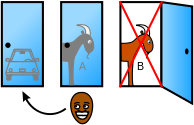
\includegraphics[width=340pt, height=200pt]{Chapters/chapter1/figures/MHproblem.png}
	%%\centerline{\epsfig{/Chapters/chapter1/figures/cat.eps,width=.8\textheight,height=.4\textwidth}}
	\caption[List of figure caption goes here]{The Monty Hall problem.}\label{fig11}
\end{figure}

Let's name $P_i$ the event \textbf{contestant picks door No. $i$}, which stays close, $H_i$ the event \textbf{host picks door No. $i$}, which is open, and there is a goat, and $C_i$ the event \textbf{car is behind door No. $i$}. In this particular setting, the contestant is interested in the probability of the event $P(C_2|H_3,P_1)$. A naive answer would be that it is irrelevant as initially $P(C_i)=1/3, \ i=1,2,3$, and now $P(C_i|H_3)=1/2, \ i=1,2$ as the host opened door No. 3. So, why bothering changing the initial guess if the odds are the same (1:1)? The important point here is that the host knows what is behind each door, and picks a door where there is a goat given contestant choice. In this particular setting, $P(H_3|C_3,P_1)=0$, $P(H_3|C_2,P_1)=1$ and $P(H_3|C_1,P_1)=1/2$. Then, using equation \ref{eq:112} 

\begin{align*}
	P(C_2|H_3,P_1)&= \frac{P(C_2,H_3,P_1)}{P(H_3,P_1)}\\
	&= \frac{P(H_3|C_2,P_1)P(C_2|P_1)P(P_1)}{P(H_3|P_1)\times P(P_1)}\\
	&= \frac{P(H_3|C_2,P_1)P(C_2)}{P(H_3|P_1)}\\
	&=\frac{1\times 1/3}{1/2},
\end{align*}
where the third equation uses the fact that $C_i$ and $P_i$ are independent events, and $P(H_3|P_1)=1/2$ due to this depending just on $P_1$ (not on $C_2$).

Therefore, changing the initial decision increases the probability of getting the car from 1/3 to 2/3! Thus, it is always a good idea to change the door.

Let's see a simulation exercise to check this answer:

\begin{tcolorbox}[enhanced,width=4.67in,center upper,
	fontupper=\large\bfseries,drop shadow southwest,sharp corners]
\textit{R code. The Monty Hall problem}
\begin{VF}
\begin{lstlisting}[ language=R]
set.seed(0101) # Set simulation seed
S <- 100000 # Simulations
Game <- function(switch = 0){
	# switch = 0 is not change  
	# switch = 1 is to change
	opts <- 1:3 
	car <- sample(opts, 1) # car location
	guess1 <- sample(opts, 1) # Initial guess 
	
	if(car != guess1) {
	 host <- opts[-c(car, guess1)]
	} else {
	 host <- sample(opts[-c(car, guess1)], 1)
	}	
	win1 <- guess1 == car # Win no change
	guess2 <- opts[-c(host, guess1)]	
	win2 <- guess2 == car # Win change
	if(switch == 0){
		win <- win1
	} else {
		win <- win2
	}
	return(win)
}

#Win probabilities not changing
Prob <- mean(replicate(S, Game(switch = 0))) 
Prob
0.3334

#Win probabilities changing
Prob <- mean(replicate(S, Game(switch = 1))) 
Prob
0.6654
\end{lstlisting}
\end{VF}
\end{tcolorbox}

\section{Bayesian framework: A brief summary of theory}\label{sec12}

For two random objects $\bm{\theta}$ and $\mathbf{y}$, the Bayes' rule may be analogously used,\footnote{From a Bayesian perspective $\mathbf{\theta}$ is fixed, but unknown. Then, it is treated as a random object despite the lack of variability (see Chapter \ref{chap2}).}

\begin{align}
	\pi(\bm{\theta}|\mathbf{y})&=\frac{p(\mathbf{y}|\bm{\theta}) \times \pi(\bm{\theta})}{p(\mathbf{y})},
	\label{eq:121}
\end{align}

where $\pi(\bm{\theta}|\mathbf{y})$ is the posterior density function, $\pi(\bm{\theta})$ is the prior density, $p(\mathbf{y}|\bm{\theta})$ is the likelihood (statistical model), and

\begin{equation}
	p(\mathbf{y})=\int_{\mathbf{\Theta}}p(\mathbf{y}|\bm{\theta})\pi(\bm{\theta})d\bm{\theta}=\mathbb{E}\left[p(\mathbf{y}|\bm{\theta})\right]
	\label{eq:121a}
\end{equation}

is the marginal likelihood or prior predictive. Observe that for this expected value to be meaningful the prior should be a proper density, that is, integrates to one, otherwise, it does not make sense. 

Observe that $p(\mathbf{y}|\bm{\theta})$ is not a density in $\bm{\theta}$. In addition, $\pi(\bm{\theta})$ does not have to integrate to 1, that is, $\pi(\bm{\theta})$ can be an improper density function, $\int_{\mathbf{\Theta}}\pi(\bm{\theta})d\bm{\theta}=\infty$. However, $\pi(\bm{\theta}|\mathbf{y})$ is a proper density function, that is, $\int_{\mathbf{\Theta}}\pi(\bm{\theta}|\mathbf{y})d\bm{\theta}=1$. For instance, set $\pi(\bm{\theta})=c$, where $c$ is a constant, then $\int_{\mathbf{\Theta}}cd\bm{\theta}=\infty$. However, $\int_{\mathbf{\Theta}}\pi(\bm{\theta}|\mathbf{y})d\bm{\theta}=\int_{\mathbf{\Theta}}\frac{p(\mathbf{y}|\bm{\theta})\times c}{\int_{\mathbf{\Theta}} p(\mathbf{y}|\bm{\theta})\times c d\bm{\theta}}d\bm{\theta}=1$ where $c$ cancels out.  

$\pi(\bm{\theta}|\mathbf{y})$ is a sample updated ``probabilistic belief" version of $\pi(\bm{\theta})$, where $\pi(\bm{\theta})$ is a prior probabilistic belief which can be constructed from previous empirical work, theory foundations, expert knowledge and/or mathematical convenience. This prior usually depends on parameters, which are named \textit{hyperparameters}. In addition, the Bayesian approach implies using a probabilistic model about $\mathbf{y}$ given $\bm{\theta}$, that is, $p(\mathbf{y}|\bm{\theta})$, where its integral over $\mathbf{\Theta}$, $p(\mathbf{y})$ is named \textit{the model evidence} due to being a measure of model fit to the data.

Observe that the Bayesian inferential approach is conditional, that is, what can we learn about an unknown object $\bm{\theta}$ given that we already observed $\mathbf{y}$? The answer is also conditional on the probabilistic model, that is $p(\mathbf{y}|\bm{\theta})$. So, what if we want to compare different models, let's say $\mathcal{M}_m$, $m=\left\{1,2,\dots,M\right\}$. Then, we should make explicit this in the Bayes' rule formulation, 

\begin{align}
	\pi(\bm{\theta}|\mathbf{y},\mathcal{M}_m)&=\frac{p(\mathbf{y}|\bm{\theta},\mathcal{M}_m) \times \pi(\bm{\theta}|\mathcal{M}_m)}{p(\mathbf{y}|\mathcal{M}_m)}.
	\label{eq:122}
\end{align}

The posterior model probability is

\begin{align}
	\pi(\mathcal{M}_m|\mathbf{y})&=\frac{p(\mathbf{y}|\mathcal{M}_m) \times \pi(\mathcal{M}_m)}{p(\mathbf{y})}, 
	\label{eq:123}
\end{align}

where $p(\mathbf{y}|\mathcal{M}_m)=\int_{\mathbf{\Theta}}p(\mathbf{y}|\bm{\theta},\mathcal{M}_m) \times \pi(\bm{\theta}|\mathcal{M}_m)d\bm{\theta}$ due to equation \ref{eq:122}, and $\pi(\mathcal{M}_m)$ is the prior model probability. 

Calculating $p(\mathbf{y})$ in equations \ref{eq:121} and \ref{eq:123} is very demanding most of the realistic cases. Fortunately, it is not required when performing inference about $\bm{\theta}$ as this is integrated out from it. Then, all what you need to know about the shape of $\bm{\theta}$ is in $p(\mathbf{y}|\bm{\theta},\mathcal{M}_m) \times \pi(\bm{\theta}|\mathcal{M}_m)$ or without explicitly conditioning on $\mathcal{M}_m$,

\begin{align}
	\pi(\bm{\theta}|\mathbf{y})& \propto p(\mathbf{y}|\bm{\theta}) \times \pi(\bm{\theta}).
	\label{eq:124}
\end{align}

Equation \ref{eq:124} is a very good shortcut to perform Bayesian inference about $\bm{\theta}$.

We also can avoid calculating $p(\mathbf{y})$ when performing model selection (hypothesis testing) using posterior odds ratio, that is, comparing models $\mathcal{M}_1$ and $\mathcal{M}_2$,

\begin{align}
	PO_{12}&=\frac{\pi(\mathcal{M}_1|\mathbf{y})}{\pi(\mathcal{M}_2|\mathbf{y})} \nonumber \\
	&=\frac{p(\mathbf{y}|\mathcal{M}_1)}{p(\mathbf{y}|\mathcal{M}_2)}\times\frac{\pi(\mathcal{M}_1)}{\pi(\mathcal{M}_2)},
	\label{eq:125}
\end{align}

where the first term in equation \ref{eq:125} is named the Bayes factor, and the second term is the prior odds. Observe that the Bayes factor is a ratio of ordinates for $\mathbf{y}$ under different models. Then, the Bayes factor is a measure of relative sample evidence in favor of model 1 compared to model 2. 

However, we still need to calculate $p(\mathbf{y}|\mathcal{M}_m)=\int_{\mathbf{\Theta}}p(\mathbf{y}|\bm{\theta},\mathcal{M}_m)\pi(\bm{\theta}|\mathcal{M}_m)d\bm{\theta}=\mathbb{E}\left[p(\mathbf{y}|\bm{\theta},\mathcal{M}_m)\right]$. For this integral to be meaningful, the prior must be proper. Using improper prior has unintended consequences when comparing models, for instance, parsimonious models are favored by posterior odds or Bayes factors depend on units of measure (see Chapter \ref{chap4}). 

A nice feature of comparing models using posterior odds is that if we have an exhaustive set of competing models such that $\sum_{m=1}^M \pi(\mathcal{M}_m|\mathbf{y})=1$, then we can recover $\pi(\mathcal{M}_m|\mathbf{y})$ without calculating $p(\mathbf{y})$. In particular, given two models $\mathcal{M}_1$ and $\mathcal{M}_2$ such that $\pi(\mathcal{M}_1|\mathbf{y})+\pi(\mathcal{M}_2|\mathbf{y})=1$. Then, $\pi(\mathcal{M}_1|\mathbf{y})=\frac{PO_{12}}{1+PO_{12}}$ and $\pi(\mathcal{M}_2|\mathbf{y})=1-\pi(\mathcal{M}_1|\mathbf{y})$. In general, $\pi(\mathcal{M}_m|\mathbf{y})=\frac{p(\mathbf{y}|\mathcal{M}_m)\times \pi(\mathcal{M}_m)}{\sum_{l=1}^M p(\mathbf{y}|\mathcal{M}_l)\times \pi(\mathcal{M}_l)}$. These posterior model probabilities can be used to perform Bayesian model averaging.

Table \ref{tab:guide} shows guidelines for the interpretation of $2\log(PO_{12})$ \cite{Kass1995}. This transformation is done to replicate the structure of the likelihood ratio test statistic. However, posterior odds do not require nested models as the likelihood ratio test does.

\begin{table}%1
	%\noautomaticrules
	\tabletitle{Kass and Raftery guidelines.}\label{tab:guide}%
	\begin{tabular}{ccc}
		\textbf{$2\times\log(PO_{12})$}    & \textbf{$PO_{12}$} & \textbf{Evidence against $\mathcal{M}_2$} \\
		\hline
		0 to 2 & 1 to 3 & Not worth more than a bare mention\\
		2 to 6 & 3 to 20 & Positive\\
		6 to 10 & 20 to 150 & Strong\\
		$> 10$  & $> 150$ & Very strong\\
	\end{tabular}
\end{table}

Observe that the posterior odds ratio is a relative criterion, that is, we specify an exhaustive set of competing models, and compare them. However, we may want to check the performance of a model in its own or use a non-informative prior. In this case, we can use \textit{the posterior predictive p-value} \cite{Gelman1996,gelman1996posterior}.\footnote{\cite{Bayarri2000} show potential issues due to using data twice in the construction of the predictive p values. They also present alternative proposals, for instance, \textit{the partial posterior predictive p value}.}

The intuition behind the predictive p-value is simple: analyze discrepancy between model's assumptions and data by checking a potential extreme tail-area probability. Observe that this approach does not check if a model is true, its focus is on potential discrepancies between a model and the data at hand. 

This is done simulating pseudo-data from our sampling model ($\mathbf{y}^{(s)}, s=1,2,\dots,S$) using draws from the posterior distribution, and then calculating a discrepancy measure, $D(\mathbf{y}^{(s)},\bm{\theta})$, to estimate the posterior predictive p-value, $p_D(\mathbf{y})=P[D(\mathbf{y}^{(s)},\bm{\theta})\geq D(\mathbf{y},\bm{\theta})]$ using the proportion of the $S$ draws for which $D(\mathbf{y}^{(s)},\bm{\theta}^{(s)})\geq D(\mathbf{y},\bm{\theta}^{(s)})$. Extreme tail probabilities ($p(D_{\mathbf{y}}) \leq 0.05  \ \text{or} \ p(D_{\mathbf{y}}) \geq 0.95$) suggest potential discrepancy between the data and the model. \cite{gelman1996posterior} also suggest the posterior predictive p-value based on the \textit{minimum discrepancy}, $D_{min}(\mathbf{y})=\min_{\bm{\theta}}D(\mathbf{y},\bm{\theta})$, and the \textit{average discrepancy} statistic $D(\mathbf{y})=\mathbb{E}[D(\mathbf{y},\bm{\theta})]=\int_{\mathbf{\Theta}}D(\mathbf{y},\bm{\theta})\pi(\mathbf{\theta|\mathbf{y}})d\bm{\theta}$. These alternatives can be more computational demanding.

The Bayesian approach is also suitable to get probabilistic predictions, that is, we can obtain a posterior predictive density 

\begin{align}
	\pi(\mathbf{Y}_0|\mathbf{y},\mathcal{M}_m) & =\int_{\mathbf{\Theta}}\pi(\mathbf{Y}_0,\bm{\theta}|\mathbf{y},\mathcal{M}_m)d\bm{\theta}\nonumber\\
	&=\int_{\mathbf{\Theta}}\pi(\mathbf{Y}_0|\bm{\theta},\mathbf{y},\mathcal{M}_m)\pi(\bm{\theta}|\mathbf{y},\mathcal{M}_m)d\bm{\theta}.
	\label{eq:126}
\end{align}

Observe that equation \ref{eq:126} is again an expectation $\mathbb{E}[\pi(\mathbf{Y}_0|\bm{\theta},\mathbf{y},\mathcal{M}_m)]$, this time using the posterior distribution. Therefore,  the Bayesian approach takes estimation error into account when performing prediction. 

As we have shown many times, expectation (integration) is a common feature in Bayesian inference. That is why the remarkable relevance of computation based on \textit{Monte Carlo integration} in the Bayesian framework (see Chapter \ref{chap5}).  

\textit{Bayesian model average} (BMA) allows considering model uncertainty in prediction or any unknown probabilistic object. In the prediction case, 

\begin{align}
	\pi(\mathbf{Y}_0|\mathbf{y})&=\sum_{m=1}^M \pi(\mathcal{M}_m|\mathbf{y})\pi(\mathbf{Y}_0|\mathbf{y},\mathcal{M}_m),
\end{align}

and parameters case,

\begin{align}
	\pi(\bm{\theta}|\mathbf{y})&=\sum_{m=1}^M \pi(\mathcal{M}_m|\mathbf{y})\pi(\bm{\theta}|\mathbf{y},\mathcal{M}_m),
\end{align}

where 

\begin{align}
	\mathbb{E}(\bm{\theta}|\mathbf{y})=\sum_{m=1}^{M}\hat{\bm{\theta}}_m \pi(\mathcal{M}_m|\mathbf{y}),
	\label{eq:127}
\end{align}

and

\begin{align}
	Var({\theta}_k|\mathbf{y})= \sum_{m=1}^{M}\pi(\mathcal{M}_m|\mathbf{y}) \widehat{Var} ({\theta}_{km}|\mathbf{y},\mathcal{M}_m)+\sum_{m=1}^{M} \pi(\mathcal{M}_m|\mathbf{y}) (\hat{{\theta}}_{km}-\mathbb{E}[{\theta}_{km}|\mathbf{y}])^2,
	\label{eq:128}
\end{align}

$\hat{\bm{\theta}}_m$ is the posterior mean and $\widehat{Var}({\theta}_{km}|\mathbf{y},\mathcal{M}_m)$ is the posterior variance of the $k$-th element of $\bm{\theta}$ under model $\mathcal{M}_m$.

Observe how the variance in equation \ref{eq:128} encloses extra variability due to potential differences between mean posterior estimates associated with each model, and the posterior mean involving model uncertainty in equation \ref{eq:127}.

A nice advantage of the Bayesian approach, which is very useful in \textit{state space representations} (see Chapter \ref{chap8}), is the way that the posterior distribution updates with new sample information. Given $\mathbf{y}=\mathbf{y}_{1:t+1}$ a sequence of observations from 1 to $t+1$, then

\begin{align}
	\pi(\bm{\theta}|\mathbf{y}_{1:t+1})&\propto p(\mathbf{y}_{1:t+1}|\bm{\theta})\times \pi(\bm{\theta})\nonumber\\
	&= p(y_{t+1}|\mathbf{y}_{1:t},\bm{\theta})\times p(\mathbf{y}_{1:t}|\bm{\theta})\times \pi(\bm{\theta})\nonumber\\
	&\propto p(y_{t+1}|\mathbf{y}_{1:t},\bm{\theta})\times \pi(\bm{\theta}|\mathbf{y}_{1:t}). 
\end{align}

We observe that the new prior is just the posterior distribution using the previous observations. This is particular useful under the assumption of \textit{conditional independence}, that is, $y_{t+1}\perp\mathbf{y}_{1:t}|\bm{\theta}$, then $p(y_{t+1}|\mathbf{y}_{1:t},\bm{\theta})=p(y_{t+1}|\bm{\theta})$ such that the posterior can be recovered recursively \cite{petris2009dynamic}. This facilities online updating due to all information up to $t$ being in $\bm{\theta}$. Then, $\pi(\bm{\theta}|\mathbf{y}_{1:t+1})\propto p(y_{t+1}|\bm{\theta})\times \pi(\bm{\theta}|\mathbf{y}_{1:t})\propto\prod_{h=1}^{t+1} p(y_h|\bm{\theta})\times \pi(\bm{\theta})$. This recursive expression can be calculated faster at some specific point in time $t$ compared to a batch mode algorithm, which requires processing simultaneously all information up to $t$.

It is also important to wonder about the sampling properties of ``Bayesian estimators". This topic has attracted attention of statisticians and econometricians long time ago. For instance, asymptotic posterior concentration at the population parameter vector is discussed by \cite{bickel1969some}. Convergence of posterior distributions is stated by the Bernstein-von Mises theorem \cite{Lehmann2003,van2000asymptotic}, which creates a link between \textit{credible intervals (sets)} and confidence intervals (sets), where a credible interval is an interval in the domain of the posterior distribution within which an unknown parameter falls with a particular probability. Credible intervals treat bounds as fixed and parameters as random, whereas confidence intervals reverse this. There are many settings in parametric models where Bayesian credible intervals with $\alpha$ level converge asymptotically to confidence intervals at $\alpha$ level. This suggests that Bayesian inference is asymptotically correct from a sampling perspective in these settings.

A heuristic approach to show this in the simplest case where we assume random sampling and $\theta\in \mathcal{R}$ is the following: $p(\mathbf{y}|\theta)=\prod_{i=1}^N p(y_i|\theta)$ such that the log likelihood is $l(\mathbf{y}|\theta)\equiv\log p(\mathbf{y}|\theta)=\sum_{i=1}^N \log p(y_i|\theta)=N\times \bar{l}(\mathbf{y}|\theta)$ where $\bar{l}\equiv\frac{1}{N}\sum_{i=1}^N \log p(y_i|\theta)$ is the mean likelihood.\footnote{Take into account that in the likelihood function the argument is $\theta$. However, we keep the notation for facility in exposition.} Then, the posterior distribution is proportional to 

\begin{align}
	\pi(\theta|\mathbf{y})&\propto p(\mathbf{y}|\theta) \times \pi(\theta)\nonumber\\
	&=\exp\left\{N\times \bar{l}(\mathbf{y}|\theta)\right\} \times \pi(\theta).
\end{align}

Observe that as the sample size gets large, that is, $N\rightarrow \infty$, the exponential term should dominate the prior distribution as long as this does not depend on $N$ such that the likelihood determines the posterior distribution asymptotically.

\textit{Maximum likelihood} theory shows that $\lim_{N\to\infty} \bar{l}(\mathbf{y}|\theta)\rightarrow \bar{l}(\mathbf{y}|\theta_0)$ where $\theta_0$ is the population parameter of the data generating process. In addition, doing a second order Taylor expansion of the log likelihood at the Maximum likelihood estimator,

\begin{align*}
	l(\mathbf{y}|\theta)&\approx l(\mathbf{y}|\hat{\theta})+\left.\frac{dl(\mathbf{y}|{\theta})}{d\theta}\right\vert_{\hat{\theta}}(\theta-\hat{\theta})+\frac{1}{2}\left.\frac{d^2l(\mathbf{y}|{\theta})}{d\theta^2}\right\vert_{\hat{\theta}}(\theta-\hat{\theta})^2\\
	&= l(\mathbf{y}|\hat{\theta})+\frac{1}{2}\left.\sum_{i=1}^N\frac{d^2l(y_i|{\theta})}{d\theta^2}\right\vert_{\hat{\theta}}(\theta-\hat{\theta})^2\\
	&= l(\mathbf{y}|\hat{\theta})-\frac{1}{2}\left.N\left[-\bar{l}''\right\vert_{\hat{\theta}}\right](\theta-\hat{\theta})^2 
\end{align*}

\begin{align*}
	&= l(\mathbf{y}|\hat{\theta})-\frac{N}{2\sigma^2}(\theta-\hat{\theta})^2\\ 
\end{align*}

where $\left.\frac{dl(\mathbf{y}|\theta)}{d\theta}\right\vert_{\hat{\theta}}=0$, $\bar{l}''\equiv\frac{1}{N}\left.\sum_{i=1}^N\frac{d^2l(y_i|{\theta})}{d\theta^2}\right\vert_{\hat{\theta}}$ and $\sigma^2:=\left[\left.-\bar{l}''\right\vert_{\hat{\theta}}\right]^{-1}$.\footnote{The last definition follows from standard theory in maximum likelihood estimation (see \cite[Chap. ~10]{casella2024statistical} and \cite[Chap. ~13]{wooldridge2010econometric}).} Then,

\begin{align*}
	\pi(\theta|\mathbf{y})&\propto \exp\left\{{l}(\mathbf{y}|\theta)\right\} \times \pi(\theta)\\
	&\approx \exp\left\{l(\mathbf{y}|\hat{\theta})-\frac{N}{2\sigma^2}(\theta-\hat{\theta})^2\right\} \times \pi(\theta)\\
	&\propto \exp\left\{-\frac{N}{2\sigma^2}(\theta-\hat{\theta})^2\right\} \times \pi(\theta)\\ 
\end{align*}

Observe that we have that the posterior density is proportional to the kernel of a normal density with mean $\hat{\theta}$ and variance $\sigma^2/N$ as long as $\pi(\hat{\theta})\neq 0$. This kernel dominates as the sample size gets large due to $N$ in the exponential term. Observe that the prior should not exclude values of $\theta$ that are logically possible, such as $\hat{\theta}$.

\subsection{Example: Health insurance}\label{sec121}

Suppose that you are analyzing to buy a health insurance next year. To make a better decision you want to know \textit{what is the probability that you visit your Doctor at least once next year?} To answer this question you have records of the number of times that you have visited your Doctor the last 5 years, $\mathbf{y}=\left\{0, 3, 2, 1, 0\right\}$. How to proceed?

Assuming that this is a random sample\footnote{Independent and identically distributed draws.} from a data generating process (statistical model) that is Poisson, that is, $Y_i\sim P(\lambda)$, and your probabilistic prior beliefs about $\lambda$ are well described by a Gamma distribution with shape and scale parameters $\alpha_0$ and $\beta_0$, $\lambda\sim G(\alpha_0, \beta_0)$, then, you are interested in calculating the probability $P(Y_0>0|\mathbf{y})$. You need to calculate the posterior predictive density $\pi(Y_0|\mathbf{y})$ to answer this question in a Bayesian way.

In this example, $p(\mathbf{y}|\lambda)$ is Poisson, and $\pi(\lambda)$ is Gamma. Then, using \ref{eq:126} 

\begin{align*}
	\pi(Y_0|\mathbf{y})=&\int_{0}^{\infty}\frac{\lambda^{y_0}\exp\left\{-\lambda\right\}}{y_0!}\times \pi(\lambda|\mathbf{y})d\lambda,\\
\end{align*}

where the posterior distribution is $\pi(\lambda|\mathbf{y})\propto \lambda^{\sum_{i=1}^N y_i + \alpha_0 - 1}\exp\left\{-\lambda\left(\frac{\beta_0 N+1}{\beta_0}\right)\right\}$ by equation \ref{eq:121}.

Observe that the last expression is the kernel of a Gamma distribution with parameters $\alpha_n=\sum_{i=1}^N y_i + \alpha_0$ and $\beta_n=\frac{\beta_0}{\beta_0 N + 1}$. Given that $\int_0^{\infty}\pi(\lambda|\mathbf{y})d\lambda=1$, then the constant of proportionality in the last expression is $\Gamma(\alpha_n)\beta_n^{\alpha_n}$, where $\Gamma(\cdot)$ is the gamma function. Thus, the posterior density function $\pi(\lambda|\mathbf{y})$ is $G(\alpha_n,\beta_n)$.

Observe that 

\begin{align*}
	\mathbb{E}[\lambda|\mathbf{y}]&=\alpha_n\beta_n\\
	&=\left(\sum_{i=1}^N y_i + \alpha_0\right)\left(\frac{\beta_0}{\beta_0 N + 1}\right)\\
	&=\bar{y}\left(\frac{N\beta_0}{N\beta_0+1}\right)+\alpha_0\beta_0\left(\frac{1}{N\beta_0+1}\right)\\
	&=w\bar{y}+(1-w)\mathbb{E}[\lambda],
\end{align*}

where $\bar{y}$ is the sample mean, which is the maximum likelihood estimator of $\lambda$ in this example, $w=\left(\frac{N\beta_0}{N\beta_0+1}\right)$ and $\mathbb{E}[\lambda]=\alpha_0\beta_0$ is the prior mean. The posterior mean is a weighted average of the maximum likelihood estimator (sample information) and the prior mean. Observe that $\lim_{N\rightarrow\infty}w= 1$, that is, the sample information asymptotically dominates.

The predictive distribution is

\begin{align*}
	\pi(Y_0|\mathbf{y})=&\int_{0}^{\infty}\frac{\lambda^{y_0}\exp\left\{-\lambda\right\}}{y_0!}\times \frac{1}{\Gamma(\alpha_n)\beta_n^{\alpha_n}}\lambda^{\alpha_n-1}\exp\left\{-\lambda/\beta_n\right\} d\lambda\\
	=&\frac{1}{y_0!\Gamma(\alpha_n)\beta_n^{\alpha_n}}\int_{0}^{\infty}\lambda^{y_0+\alpha_n-1}\exp\left\{-\lambda\left(\frac{1+\beta_n}{\beta_n}\right)\right\}d\lambda\\
	=&\frac{\Gamma(y_0+\alpha_n)\left(\frac{\beta_n}{\beta_n+1}\right)^{y_0+\alpha_n}}{y_0!\Gamma(\alpha_n)\beta_n^{\alpha_n}}\\
	=&{y_0+\alpha_n-1 \choose y_0}\left(\frac{\beta_n}{\beta_n+1}\right)^{y_0}\left(\frac{1}{\beta_n+1}\right)^{\alpha_n}.
\end{align*}

The third equality follows from the kernel of a Gamma density, and the fourth from ${y_0+\alpha_n-1 \choose y_0}=\frac{(y_0+\alpha_n-1)(y_0+\alpha_n-2)\dots\alpha_n}{y_0!}=\frac{\Gamma(y_0+\alpha_n)}{\Gamma(\alpha_n)y_0!}$ using a property of the Gamma function.

Observe that this is a Negative Binomial density, that is $Y_0|\mathbf{y}\sim NB(\alpha_n,p_n)$ where $p_n=\frac{\beta_n}{\beta_n+1}$. 

Up to this point, we have said nothing about the hyperparameters, which are required to give a concrete response to this exercise. Thus, we show two approaches to set them. First, we set $\alpha_0=0.001$ and $\beta_0=1/0.001$ which imply vague prior information about $\lambda$ due to having a large degree of variability compared to the mean information.\footnote{We should be aware that there may be technical problems using this king of hyperparameters in this setting \cite{gelman2006prior}.} In particular, $\mathbb{E}[\lambda]=1$ and $\mathbb{V}ar[\lambda]=1000$. 

In this setting, $P(Y_0>0|\mathbf{y})=1-P(Y_0=0|\mathbf{y})\approx 0.67$. That is, the probability of visiting the Doctor at least once next year is approximately 0.67.

Another approach is using \textit{Empirical Bayes}, where we set the hyperparameters maximizing the logarithm of the marginal likelihood, that is, $\left[\hat{\alpha}_0 \ \hat{\beta}_0\right]^{\top}=\underset{\alpha_0 ,\beta_0}{\mathrm{argmax}} \ \ln p(\mathbf{y})$ where

\begin{align*}
	p(\mathbf{y})&=\int_0^{\infty}\left\{\frac{1}{\Gamma(\alpha_0)\beta_0^{\alpha_0}}\lambda^{\alpha_0-1}\exp\left\{-\lambda/\beta_0\right\} \prod_{i=1}^N\frac{\lambda^{y_i}\exp\left\{-\lambda\right\}}{ y_i!}\right\}d\lambda\\
	&=\frac{\int_0^{\infty}\lambda^{\sum_{i=1}^N y_i+\alpha_0-1}\exp\left\{-\lambda \left(\frac{\beta_0 N +1}{\beta_0}\right) \right\}d\lambda}{\Gamma(\alpha_0)\beta_0^{\alpha_0}\prod_{i=1}^N y_i!}\\
	&=\frac{\Gamma(\sum_{i=1}^N y_i+\alpha_0)\left(\frac{\beta_0}{N\beta_0+1}\right)^{\sum_{i=1}^N y_i}\left(\frac{1}{N\beta_0+1}\right)^{\alpha_0}}{\Gamma(\alpha_0)\prod_{i=1}^N y_i}
\end{align*}

Using the empirical Bayes approach, we get $\hat{\alpha}_0=51.8$ and $\hat{\beta}_0=0.023$, then $P(Y_0>0|\mathbf{y})=1-P(Y_0=0|\mathbf{y})\approx 0.70$.

Observe that we can calculate the posterior odds comparing the model using an Empirical Bayes prior (model 1) versus the vague prior (model 2). We assume that $\pi(\mathcal{M}_1)=\pi(\mathcal{M}_2)=0.5$, then

\begin{align*}
	PO_{12}&=\frac{p(\mathbf{y}|\text{Empirical Bayes})}{p(\mathbf{y}|\text{Vague prior})}\\
	&=\frac{\frac{\Gamma(\sum_{i=1}^N y_i+51.807)\left(\frac{0.023}{N\times 0.023+1}\right)^{\sum_{i=1}^N y_i}\left(\frac{1}{N\times 0.023+1}\right)^{51.807}}{\Gamma(51.807)}}{\frac{\Gamma(\sum_{i=1}^N y_i+0.001)\left(\frac{1/0.001}{N/0.001+1}\right)^{\sum_{i=1}^N y_i}\left(\frac{1}{N/0.001+1}\right)^{0.001}}{\Gamma(0.001)}}\\
	&\approx 919.
\end{align*}

Then, $2\times \log(PO_{12})=13.64$, there is very strong evidence against the vague prior model (see Table \ref{tab:guide}). In particular, $\pi(\text{Empirical Bayes}|\mathbf{y})=\frac{919}{1+919}=0.999$ and $\pi(\text{Vague prior}|\mathbf{y})=1-0.999=0.001$. These probabilities can be used to perform Bayesian model average (BMA). In particular,

\begin{align*}
	\mathbb{E}(\lambda|\mathbf{y})&=1.2\times 0.999+1.2\times 0.001=1.2\\
	Var(\lambda|\mathbf{y})&=0.025\times 0.999+0.24\times 0.001\\
	& + (1.2-1.2)^2\times 0.999 + (1.2-1.2)^2\times 0.001= 0.025.
\end{align*}

The BMA predictive distribution is a mix of negative binomial distributions, that is, $y_0|\mathbf{y}\sim 0.999\times NB(57.8, 0.02)+0.001\times NB(6.001, 0.17)$.

\begin{tcolorbox}[enhanced,width=4.67in,center upper,
	fontupper=\large\bfseries,drop shadow southwest,sharp corners]
\textit{R code. Health insurance, predictive distribution using vague hyperparameters}
\begin{VF}
\begin{lstlisting}[ language=R]
set.seed(010101)
y <- c(0, 3, 2, 1, 0) # Data
N <- length(y)
ProbBo <- function(y, a0, b0){
	N <- length(y)
	#sample size
	an <- a0 + sum(y) 
	# Posterior shape parameter
	bn <- b0 / ((b0 * N) + 1) 
	# Posterior scale parameter
	p <- bn / (bn + 1) 
	# Probability negative binomial density
	Pr <- 1 - pnbinom(0, size=an,prob=(1 - p)) 
	# Probability of visiting the Doctor at least once next year
	# Observe that in R there is a slightly different parametrization.
	return(Pr)
} 
# Using a vague prior:
a0 <- 0.001 # Prior shape parameter
b0 <- 1 / 0.001 # Prior scale parameter
PriMeanV <- a0 * b0 # Prior mean
PriVarV <- a0 * b0^2 # Prior variance
Pp <- ProbBo(y, a0 = 0.001, b0 = 1 / 0.001) 
# This setting is vague prior information.
Pp
0.67
\end{lstlisting}
\end{VF}
\end{tcolorbox} 

\begin{tcolorbox}[enhanced,width=4.67in,center upper,
	fontupper=\large\bfseries,drop shadow southwest,sharp corners]
\textit{R code. Health insurance, predictive distribution using empirical Bayes}
\begin{VF}
\begin{lstlisting}[ language=R]
# Using Empirical Bayes
LogMgLik <- function(theta, y){
 N <- length(y) 
 #sample size
 a0 <- theta[1] 
 # prior shape hyperparameter
 b0 <- theta[2] 
 # prior scale hyperparameter
 an <- sum(y) + a0 
 # posterior shape parameter
 if(a0 <= 0 || b0 <= 0){ 
  #Avoiding negative values
  lnp <- -Inf
  }else{
  lnp <- lgamma(an) + sum(y)*log(b0/(N*b0+1)) - a0*log(N*b0+1) - lgamma(a0)
 } 
 # log marginal likelihood
 return(-lnp)
}			
theta0 <- c(0.01, 1/0.1) 
# Initial values
control <- list(maxit = 1000) 
# Number of iterations in optimization
EmpBay <- optim(theta0, LogMgLik, method = "BFGS", control = control, hessian = TRUE, y = y) 
# Optimization
EmpBay$convergence
0
a0EB <- EmpBay$par[1] 
# Prior shape using empirical Bayes
a0EB
51.81
b0EB <- EmpBay$par[2] 
# Prior scale using empirical Bayes
b0EB
0.023
PriMeanEB <- a0EB * b0EB 
# Prior mean
PriVarEB <- a0EB * b0EB^2 
# Prior variance
PpEB <- ProbBo(y, a0 = a0EB, b0 = b0EB) 
# This setting is using emprical Bayes.
PpEB
0.70 
\end{lstlisting}
\end{VF}
\end{tcolorbox} 

\begin{tcolorbox}[enhanced,width=4.67in,center upper,
	fontupper=\large\bfseries,drop shadow southwest,sharp corners]
	\textit{R code. Health insurance, density plots}
\begin{VF}
\begin{lstlisting}[ language=R]		
# Density figures: 
# This code helps plotting densities
lambda <- seq(0.01, 10, 0.01) 
# Values of lambda
VaguePrior <- dgamma(lambda,shape=a0,scale = b0)
EBPrior <- dgamma(lambda,shape=a0EB,scale = b0EB)
PosteriorV <- dgamma(lambda, shape = a0 + sum(y), scale = b0 / ((b0 * N) + 1)) 
PosteriorEB <- dgamma(lambda, shape = a0EB+sum(y), scale = b0EB / ((b0EB * N) + 1))			
# Likelihood function
Likelihood <- function(theta, y){
 LogL <- dpois(y, theta, log = TRUE)
 Lik <- prod(exp(LogL))
 return(Lik)
}
Liks <- sapply(lambda, function(par) {Likelihood(par, y = y)})
Sc <- max(PosteriorEB)/max(Liks) 
#Scale for displaying in figure
LiksScale <- Liks * Sc
data <- data.frame(cbind(lambda, VaguePrior, EBPrior, PosteriorV, PosteriorEB, LiksScale)) #Data frame
require(ggplot2) # Cool figures
require(latex2exp) # LaTeX equations in figures
require(ggpubr) # Multiple figures in one page
fig1 <- ggplot(data = data, aes(lambda, VaguePrior)) + geom_line() + 	xlab(TeX("$\\lambda$")) + ylab("Density") +	ggtitle("Prior: Vague Gamma") 
fig2 <- ggplot(data = data, aes(lambda, EBPrior)) + geom_line() + xlab(TeX("$\\lambda$")) + ylab("Density") + ggtitle("Prior: Empirical Bayes Gamma")
fig3 <- ggplot(data = data, aes(lambda, PosteriorV)) + geom_line() + xlab(TeX("$\\lambda$")) + ylab("Density") + ggtitle("Posterior: Vague Gamma")
fig4 <- ggplot(data = data, aes(lambda, PosteriorEB)) + geom_line() + xlab(TeX("$\\lambda$")) + ylab("Density") + ggtitle("Posterior: Empirical Bayes Gamma")
FIG <- ggarrange(fig1, fig2, fig3, fig4, ncol = 2, nrow = 2)
annotate_figure(FIG, top = text_grob("Vague versus Empirical Bayes: Poisson-Gamma model", color = "black", face = "bold", size = 14))
dataNew <- data.frame(cbind(rep(lambda, 3), c(EBPrior, PosteriorEB, LiksScale), rep(1:3, each = 1000))) #Data frame
colnames(dataNew) <- c("Lambda", "Density", "Factor")
dataNew$Factor <- factor(dataNew$Factor, levels=c("1", "3", "2"), 
labels=c("Prior", "Likelihood", "Posterior"))
ggplot(data = dataNew, aes_string(x = "Lambda", y = "Density", group = "Factor")) + geom_line(aes(color = Factor)) + xlab(TeX("$\\lambda$")) + ylab("Density") + ggtitle("Prior, likelihood and posterior: Empirical Bayes Poisson-Gamma model") + guides(color=guide_legend(title="Information")) + scale_color_manual(values = c("red", "yellow", "blue"))
\end{lstlisting}
\end{VF}
\end{tcolorbox} 

\begin{figure}[!h]
	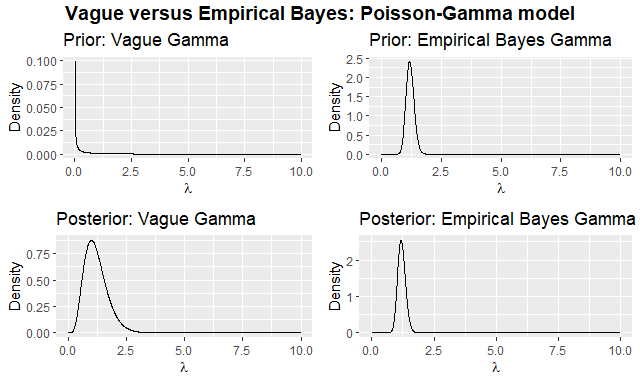
\includegraphics[width=340pt, height=200pt]{Chapters/chapter1/figures/PoisGam.png}
	%%\centerline{\epsfig{/Chapters/chapter1/figures/cat.eps,width=.8\textheight,height=.4\textwidth}}
	\caption[List of figure caption goes here]{Vague versus Empirical Bayes: Poisson-Gamma model.}\label{fig12}
\end{figure}

\begin{figure}[!h]
	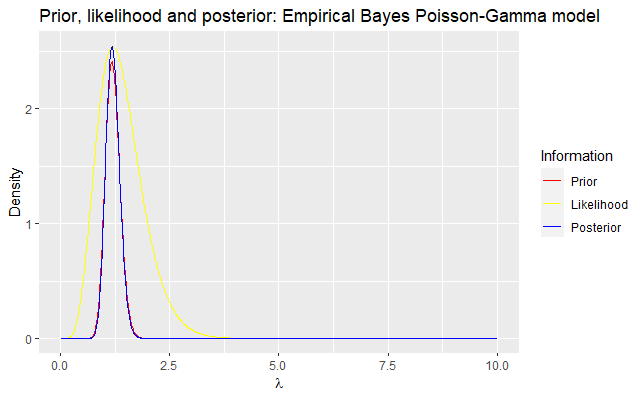
\includegraphics[width=340pt, height=200pt]{Chapters/chapter1/figures/PriorLikPost.png}
	%%\centerline{\epsfig{/Chapters/chapter1/figures/cat.eps,width=.8\textheight,height=.4\textwidth}}
	\caption[List of figure caption goes here]{Prior, likelihood and posterior: Empirical Bayes Poisson-Gamma model.}\label{fig13}
\end{figure}

Figure \ref{fig12} displays prior and posterior densities based on vague and Empirical Bayes hyperparameters. We see that prior and posterior densities using the latter are more informative as expected.

Figure \ref{fig13} shows the prior, scaled likelihood and posterior densities of $\lambda$ based on the hyperparameters of the Empirical Bayes approach. The posterior density is a compromise between prior and sample information. 

\clearpage
\begin{tcolorbox}[enhanced,width=4.67in,center upper,
	fontupper=\large\bfseries,drop shadow southwest,sharp corners]
\textit{R code. Health insurance, Predictive density}
\begin{VF}
\begin{lstlisting}[
	 language=R]
# Predictive distributions
PredDen <- function(y, y0, a0, b0){
	N <- length(y)
	#sample size
	an <- a0 + sum(y) 
	# Posterior shape parameter
	bn <- b0 / ((b0 * N) + 1) 
	# Posterior scale parameter
	p <- bn / (bn + 1) 
	# Probability negative binomial density
	Pr <- dnbinom(y0, size=an, prob=(1 - p))
	# Predictive density
	# Observe that in R there is a slightly different parametrization.
	return(Pr)
}
y0 <- 0:10
PredVague <- PredDen(y=y, y0=y0, a0=a0, b0=b0)
PredEB <- PredDen(y=y, y0=y0, a0=a0EB, b0=b0EB)
dataPred <- as.data.frame(cbind(y0, PredVague, PredEB))
colnames(dataPred) <- c("y0", "PredictiveVague", "PredictiveEB")
ggplot(data = dataPred) + geom_point(aes(y0, PredictiveVague, color = "red")) +  
xlab(TeX("$y_0$")) + ylab("Density") + ggtitle("Predictive density: Vague and Empirical Bayes priors") + geom_point(aes(y0, PredictiveEB, color = "yellow")) +
guides(color = guide_legend(title="Prior")) + scale_color_manual(labels = c("Vague", "Empirical Bayes"), values = c("red", "yellow")) + scale_x_continuous(breaks=seq(0,10,by=1))
\end{lstlisting}
\end{VF}
\end{tcolorbox}

\begin{figure}[!h]
	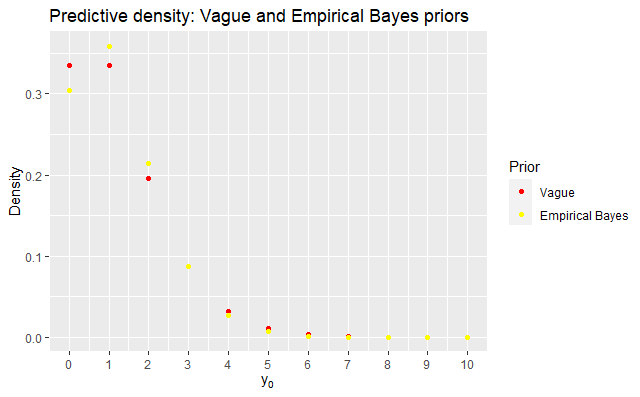
\includegraphics[width=340pt, height=200pt]{Chapters/chapter1/figures/Predictive.png}
	%%\centerline{\epsfig{/Chapters/chapter1/figures/cat.eps,width=.8\textheight,height=.4\textwidth}}
	\caption[List of figure caption goes here]{Predictive density: Vague and Empirical Bayes.}\label{fig14}
\end{figure}

Figure \ref{fig14} displays the predictive probability mass of not having any visits to a physician the next year, having one, two, and so on using Empirical Bayes and vague hyperparameters. The predictive probability of not having any visits are approximately equal to 30\% and 33\% based on the Empirical Bayes and vague hyperparameters. 

\begin{tcolorbox}[enhanced,width=4.67in,center upper,
	fontupper=\large\bfseries,drop shadow southwest,sharp corners]
\textit{R code. Health insurance, Bayesian model average}
\begin{VF}
\begin{lstlisting}[language=R]
# Posterior odds: Vague vs Empirical Bayes
PO12 <- exp(-LogMgLik(c(a0EB, b0EB), y = y))/exp(-LogMgLik(c(a0, b0), y = y))
PO12
919
PostProMEM <- PO12/(1 + PO12) 
PostProMEM
0.998
# Posterior model probability Empirical Bayes
PostProbMV <- 1 - PostProMEM 
PostProbMV
0.002
# Posterior model probability vague prior
# Bayesian model average (BMA)
PostMeanEB <- (a0EB + sum(y)) * (b0EB / (b0EB * N + 1)) 
# Posterior mean Empirical Bayes 
PostMeanV <- (a0 + sum(y)) * (b0 / (b0 * N + 1)) 
# Posterior mean vague priors
BMAmean <- PostProMEM * PostMeanEB + PostProbMV * PostMeanV  
BMAmean
1.2
# BMA posterior mean
PostVarEB <- (a0EB + sum(y)) * (b0EB/(b0EB * N + 1))^2 
# Posterior variance Empirical Bayes
PostVarV <- (a0 + sum(y)) * (b0 / (b0 * N + 1))^2 
# Posterior variance vague prior 
BMAVar <- PostProMEM * PostVarEB + PostProbMV*PostVarV + PostProMEM * (PostMeanEB - BMAmean)^2 + PostProbMV * (PostMeanV - BMAmean)^2
# BMA posterior variance   
BMAVar
0.025    
\end{lstlisting}
\end{VF}
\end{tcolorbox}

\begin{tcolorbox}[enhanced,width=4.67in,center upper,
	fontupper=\large\bfseries,drop shadow southwest,sharp corners]
	\textit{R code. Health insurance, Bayesian model average}
	\begin{VF}
		\begin{lstlisting}[ language=R]
# BMA: Predictive
BMAPred <- PostProMEM * PredEB+PostProbMV * PredVague
dataPredBMA <- as.data.frame(cbind(y0, BMAPred))
colnames(dataPredBMA) <- c("y0", "PredictiveBMA")
ggplot(data = dataPredBMA) + geom_point(aes(y0, PredictiveBMA, color = "red")) +  xlab(TeX("$y_0$")) + ylab("Density") + ggtitle("Predictive density: BMA") + guides(color = guide_legend(title="BMA")) + scale_color_manual(labels = c("Probability"), values = c("red")) + scale_x_continuous(breaks=seq(0,10,by=1)) 
		\end{lstlisting}
	\end{VF}
\end{tcolorbox}

\begin{figure}[!h]
	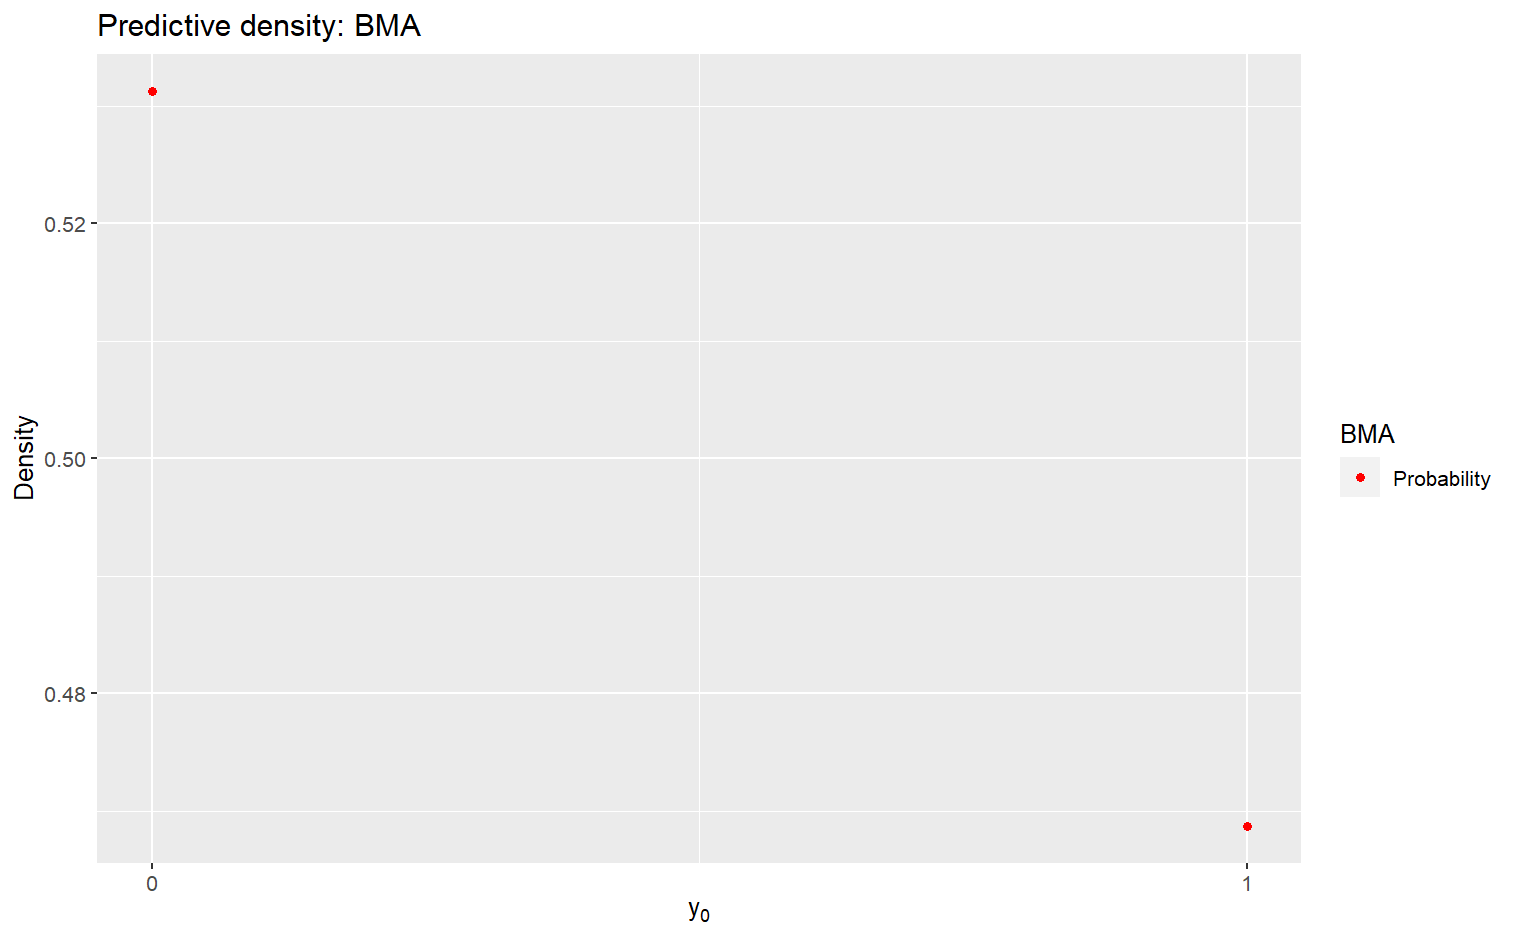
\includegraphics[width=340pt, height=200pt]{Chapters/chapter1/figures/BMA.png}
	%%\centerline{\epsfig{/Chapters/chapter1/figures/cat.eps,width=.8\textheight,height=.4\textwidth}}
	\caption[List of figure caption goes here]{Bayesian model average: Predictive density.}\label{fig15}
\end{figure}

\begin{figure}[!h]
	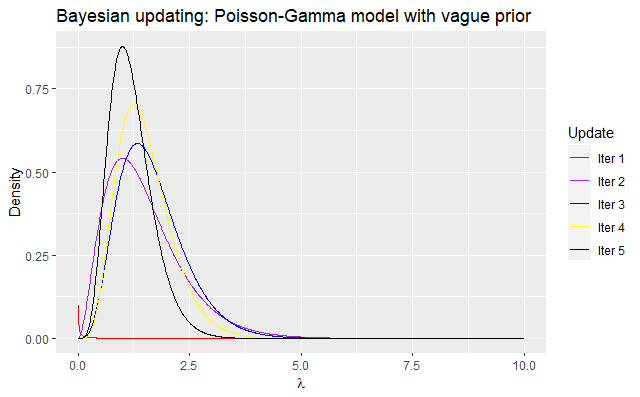
\includegraphics[width=340pt, height=200pt]{Chapters/chapter1/figures/Updating.png}
	%%\centerline{\epsfig{/Chapters/chapter1/figures/cat.eps,width=.8\textheight,height=.4\textwidth}}
	\caption[List of figure caption goes here]{Bayesian updating: Posterior densities.}\label{fig16}
\end{figure}

Figure \ref{fig15} displays the predictive density using Bayesian model average based on the vague and Empirical Bayes hyperparameters. This figure essentially resembles the predictive probability mass function based on the Empirical Bayes framework, as the posterior model probability for that setting is nearly one.

Figure \ref{fig16} displays how the posterior distribution updates given new sample information based on an initial non-informative prior (iteration 1). We see that iteration 5 is based on all the sample information in our example, as a consequence, the posterior density in iteration 5 is equal to the posterior density in Figure \ref{fig13}.

\begin{tcolorbox}[enhanced,width=4.67in,center upper,
	fontupper=\large\bfseries,drop shadow southwest,sharp corners]
\textit{R code. Health insurance, Bayes updating}
\begin{VF}
\begin{lstlisting}[ language=R]
# Bayesian updating
BayUp <- function(y, lambda, a0, b0){
	N <- length(y)
	#sample size
	an <- a0 + sum(y) 
	# Posterior shape parameter
	bn <- b0 / ((b0 * N) + 1) 
	# Posterior scale parameter
	p <- dgamma(lambda, shape = an, scale = bn) 
	# Posterior density
	return(list(Post = p, a0New = an, b0New = bn))
}
PostUp <- NULL
for(i in 1:N){
	if(i == 1){
		PostUpi <- BayUp(y[i], lambda, a0 = 0.001, b0 = 1/0.001)}
	else{
		PostUpi <- BayUp(y[i], lambda, a0 = PostUpi$a0New, b0 = PostUpi$b0New)
	}
	PostUp <- cbind(PostUp, PostUpi$Post)
}
DataUp <- data.frame(cbind(rep(lambda, 5), c(PostUp), rep(1:5, each = 1000))) #Data frame
colnames(DataUp) <- c("Lambda", "Density", "Factor")
DataUp$Factor <- factor(DataUp$Factor, levels=c("1", "2", "3", "4", "5"), 
labels=c("Iter 1", "Iter 2", "Iter 3", "Iter 4", "Iter 5"))
ggplot(data = DataUp, aes_string(x = "Lambda", y = "Density", group = "Factor")) + geom_line(aes(color = Factor)) + xlab(TeX("$\\lambda$")) + ylab("Density") + ggtitle("Bayesian updating: Poisson-Gamma model with vague prior") + guides(color=guide_legend(title="Update")) + scale_color_manual(values = c("red", "purple", "blue", "yellow", "black"))
S <- 100000 # Posterior draws
PostMeanLambdaUps <- sapply(1:N, function(i) {mean(sample(lambda, S, replace = TRUE, prob = PostUp[ , i]))}) #Posterior mean update i
paste("Posterior means using all information and sequential updating are:", round(PostMeanV, 2), "and", round(PostMeanLambdaUps[5], 2), sep = " ")
Posterior means using all information and sequential updating are: 1.2 and 1.2 
PostVarLambdaUps <- sapply(1:N, function(i) {var(sample(lambda, S, replace = TRUE, prob = PostUp[ , i]))}) #Posterior variance update i
paste("Posterior variances using all information and sequential updating are:", round(PostVarV, 2), "and", round(PostVarLambdaUps[5], 2), sep = " ")
Posterior variances using all information and sequential updating are: 0.24 and 0.24
\end{lstlisting}
\end{VF}
\end{tcolorbox}

\section{Bayesian reports: Decision theory under uncertainty}\label{sec14}

The Bayesian framework allows reporting the full posterior distributions. However, some situations demand to report a specific value of the posterior distribution (point estimate), an informative interval (set), point or interval predictions and/or selecting a specific model. Decision theory offers an elegant framework to make a decision regarding what are the optimal posterior values to report \cite{berger2013statistical}.

The point of departure is a \textit{loss function}, which is a non-negative real value function whose arguments are the unknown \textit{state of nature} ($\mathbf{\Theta}$), and a set of \textit{actions} to be made ($\mathcal{A}$), that is, 
\begin{equation*}
	L(\bm{\theta}, a):\mathbf{\Theta}\times \mathcal{A}\rightarrow \mathcal{R}^+.
\end{equation*}

This function is a mathematical expression of the loss of making mistakes. In particular, selecting action $a\in\mathcal{A}$ when $\bm{\theta}\in\mathbf{\Theta}$ is the true. In our case, the unknown state of nature can be parameters, functions of them, future or unknown realizations, models, etc.

From a Bayesian perspective, we should choose the action that minimizes the posterior expected loss ($a^*(\mathbf{y})$), that is, the \textit{posterior risk function} ($\mathbb{E}[L(\bm{\theta}, a)|\mathbf{y}]$),

\begin{equation*}
	a^*(\mathbf{y})=\underset{a \in \mathcal{A}}{\mathrm{argmin}} \  \mathbb{E}[L(\bm{\theta}, a)|\mathbf{y}], 
\end{equation*}

where $\mathbb{E}[L(\bm{\theta}, a)|\mathbf{y}]= \int_{\mathbf{\Theta}} L(\bm{\theta}, a)\pi(\bm{\theta}|\mathbf{y})d\bm{\theta}$.\footnote{\cite{Chernozhukov2003} propose Laplace type estimators (LTE) based on the \textit{quasi-posterior}, $p(\bm{\theta})=\frac{\exp\left\{L_n(\bm{\theta})\right\}\pi(\bm{\theta})}{\int_{\mathbf{\Theta}}\exp\left\{L_n(\bm{\theta})\right\}\pi(\bm{\theta})d\theta}$ where $L_n(\bm{\theta})$ is not necessarily a log-likelihood function. The LTE minimizes the \textit{quasi-posterior risk}.}

Different loss functions imply different optimal decisions. We illustrate this assuming $\theta \in \mathcal{R}$.

\begin{itemize}
	\item The quadratic loss function, $L({\theta},a)=[{\theta}-a]^2$, gives as optimal decision the posterior mean, $a^*(\mathbf{y})=\mathbb{E}[{\theta}|\mathbf{y}]$, that is 
		
	\begin{equation*}
		\mathbb{E}[{\theta}|\mathbf{y}] = \underset{a \in \mathcal{A}}{\mathrm{argmin}} \  \int_{{\Theta}} [{\theta}-a]^2\pi({\theta}|\mathbf{y})d{\theta}.
	\end{equation*}
	
	To get this results, let's use the first condition order, differentiate the risk function with respect to $a$, interchange differential and integral order, and set this equal to zero, $-2\int_{{\Theta}} [{\theta}-a^*]\pi({\theta}|\mathbf{y})d{\theta}=0$ implies that $a^*\int_{{\Theta}} \pi({\theta}|\mathbf{y})d{\theta}=a^*(\mathbf{y})=\int_{{\Theta}} {\theta}\pi({\theta}|\mathbf{y})d{\theta}=\mathbb{E}[{\theta}|\mathbf{y}]$, that is, the posterior mean is the Bayesian optimal action. This means that we should report the posterior mean as a point estimate of $\theta$ when facing the quadratic loss function.
	
	\item The generalized quadratic loss function,  $L({\theta},a)=w({\theta})[{\theta}-a]^2$, where $w({\theta})>0$ is a weighting function, gives as optimal decision rule the weighted mean. We should follow same steps as the previous result to get   $a^*(\mathbf{y})=\frac{\mathbb{E}[w({\theta})\times{\theta}|\mathbf{y}]}{\mathbb{E}[w({\theta})|\mathbf{y}]}$. Observe that the weighted average is driven by the weighting function $w({\theta})$.
	
	\item The absolute error loss function, $L({\theta},a)=|{\theta}-a|$, gives as optimal action the posterior median (Exercise 5).
	
	\item The generalized absolute error function,
	
	\begin{equation*}
		L(\theta,a)=\begin{Bmatrix} K_0(\theta-a), \theta-a\geq 0\\
			K_1(a-\theta), \theta-a < 0 \end{Bmatrix}, \ K_0,K_1>0,
	\end{equation*}
	
	implies the following risk function,
	
	\begin{align*}
		\mathbb{E}[L(\theta, a)|\mathbf{y}]&=\int_{-\infty}^a K_1(a-\theta)\pi(\theta|\mathbf{y})d\theta + \int_a^{\infty} K_0(\theta-a)\pi(\theta|\mathbf{y})d\theta. 
	\end{align*}
	
	Differentiating with respect to $a$, interchanging differentials and integrals, and equating to zero,
	\begin{align*}
		K_1\int_{-\infty}^{a^*} \pi(\theta|\mathbf{y})d\theta-K_0\int_{a^*}^{\infty} \pi(\theta|\mathbf{y})d\theta&=0,
	\end{align*}
	
	then, $\int_{-\infty}^{a^*} \pi(\theta|\mathbf{y})d\theta=\frac{K_0}{K_0+K_1}$, that is, any $K_0/(K_0+K_1)$-percentile of $\pi(\theta|\mathbf{y})$ is an optimal Bayesian estimate of $\theta$. 
\end{itemize}

We can also use decision theory under uncertainty in hypothesis testing. In particular, testing $H_0:\theta\in\Theta_0$ versus $H_1:\theta\in\Theta_1$, $\Theta=\Theta_0 \cup \Theta_1$ and $\emptyset=\Theta_0 \cap \Theta_1$, there are two actions of interest, $a_0$ and $a_1$, where $a_j$ denotes no rejecting $H_j$, $j=\left\{0,1\right\}$. 

Given the $0-K_j$ loss function,

\begin{equation*}
	L(\theta,a_j)=\begin{Bmatrix} 0, & \theta\in\Theta_j\\
		K_j, & \theta\in\Theta_j, j\neq i \end{Bmatrix},
\end{equation*}

where there is no loss if the right decision is made, for instance, no rejecting $H_0$ when $\theta\in\Theta_0$, and the loss is $K_j$ when an error is made, for instance, type I error, rejecting the null hypothesis ($H_0$) when it is true ($\theta\in\Theta_0$), implies a loss equal to $K_1$ due to picking $a_1$, no rejecting $H_1$. 

The posterior expected loss associated with decision $a_j$, that is, no rejecting $H_j$, is $\mathbb{E}[L(\theta,a_j)|\mathbf{y}]=0\times P(\Theta_j|\mathbf{y}) + K_jP(\Theta_i|\mathbf{y})=K_jP(\Theta_i|\mathbf{y})$, $j\neq i$. Therefore, the Bayes optimal decision is the one that gives the smallest posterior expected loss, that is, the null hypothesis is rejected ($a_1$ is not rejected), when $K_0P(\Theta_1|\mathbf{y}) > K_1P(\Theta_0|\mathbf{y})$. Given our framework $(\Theta=\Theta_0 \cup \Theta_1, \emptyset=\Theta_0 \cap \Theta_1)$, then $P(\Theta_0|\mathbf{y})=1-P(\Theta_1|\mathbf{y})$, and as a consequence, $P(\Theta_1|\mathbf{y})>\frac{K_1}{K_1+K_0}$, that is, the rejection region of the Bayesian test is $R=\left\{\mathbf{y}:P(\Theta_1|\mathbf{y})>\frac{K_1}{K_1+K_0}\right\}$.

Decision theory also helps to construct interval (region) estimates. Let $\Theta_{C(\mathbf{y})}\subset \Theta$ a \textit{credible set} for $\theta$, and $L(\theta,\Theta_{C(\mathbf{y})})=1-\mathbbm{1}\left\{\theta\in \Theta_{C(\mathbf{y})}\right\}$, where 

\begin{equation*}
	\mathbbm{1}\left\{\theta\in \Theta_{C(\mathbf{y})}\right\}=\begin{Bmatrix}1, & \theta\in \Theta_{C(\mathbf{y})}\\  
		0, & \theta\notin \Theta_{C(\mathbf{y})}
	\end{Bmatrix}.
\end{equation*}

Then,

\begin{equation*}
	L(\theta,\Theta_{C(\mathbf{y})})=\begin{Bmatrix}0, & \theta\in \Theta_{C(\mathbf{y})}\\  
		1, & \theta\notin \Theta_{C(\mathbf{y})}
	\end{Bmatrix},
\end{equation*}

where the 0--1 loss function is equal to zero if $\theta\in \Theta_{C(\mathbf{y})}$, and one if $\theta\notin \Theta_{C(\mathbf{y})}$. Then, the risk function is $1-P(\theta\in \Theta_{C(\mathbf{y})})$.

Given a \textit{measure of credibility} ($\alpha(\mathbf{y})$) that defines the level of trust that $\theta\in \Theta_{C(\mathbf{y})}$; then, we can measure the accuracy of the report by $L(\theta, \alpha(\mathbf{y}))=[\mathbbm{1}\left\{\theta\in \Theta_{C(\mathbf{y})}\right\}-\alpha(\mathbf{y})]^2$. This loss function could be used to suggest a choice of the report $\alpha(\mathbf{y})$. Given that this is a quadratic loss function, the optimal action is the posterior mean, that is $\mathbb{E}[\mathbbm{1}\left\{\theta\in \Theta_{C(\mathbf{y})}\right\}|\mathbf{y}]=P(\theta\in \Theta_{C(\mathbf{y})}|\mathbf{y})$. This probability can be calculated given the posterior distribution, that is, $P(\theta\in \Theta_{C(\mathbf{y})}|\mathbf{y})=\int_{\Theta_{C(\mathbf{y})}}\pi(\theta|\mathbf{y})d\theta$. This is a measure of the belief that $\theta\in \Theta_{C(\mathbf{y})}$ given the prior beliefs and sample information.

The set $\Theta_{C(\mathbf{y})}\in\Theta$ is a $100(1-\alpha)\%$ credible set with respect to $\pi(\theta|\mathbf{y})$ if $P(\theta\in \Theta_{C(\mathbf{y})}|\mathbf{y})=\int_{\Theta_{C(\mathbf{y})}}\pi(\theta|\mathbf{y})=1-\alpha$.

Two alternatives to report credible sets are the \textit{symmetric credible set} and the \textit{highest posterior density set} (HPD). The former is based on $\frac{\alpha}{2}$\% and $(1-\frac{\alpha}{2})$\% percentiles of the posterior distribution, and the latter is a $100(1-\alpha)\%$ credible interval for $\theta$ with the property that it has the smallest distance compared to any other $100(1-\alpha)\%$ credible interval for $\theta$ based on the posterior distribution. That is, $C(\mathbf{y})=\left\{\theta:\pi(\theta|\mathbf{y})\geq k(\alpha)\right\}$, where $k(\alpha)$ is the largest number such that $\int_{\theta:\pi(\theta|\mathbf{y})\geq k(\alpha)}\pi(\theta|\mathbf{y})d\theta=1-\alpha$. The HPD set can be a collection of disjoint intervals when working with multimodal posterior densities. In addition, they have the limitation of not necessary being invariant under transformations. 

Decision theory can also be used to perform prediction (point, sets or probabilistic). Suppose that there is a loss function $L(Y_0,a)$ involving the prediction of $Y_0$. Then, $\mathbb{E}_{Y_0}[L(Y_0,a)]=\int_{\mathcal{Y}_0}L(Y_0,a)\pi(Y_0|\mathbf{y})dY_0$, where $\pi(Y_0|\mathbf{y})$ is the predictive density function. Thus, we make an optimal choice for prediction that minimizes the risk function given a specific loss function.

Although BMA allows incorporating model uncertainty in a regression framework, sometimes it is desirable to select just one model. A compelling alternative is the model with the highest posterior model probability. This model is the best alternative for prediction in the case of a 0--1 loss function \cite{Clyde2004}.

\subsection{Example: Health insurance continues}\label{131}

We show some optimal rules in the health insurance example. In particular, the best point estimates of $\lambda$ given the quadratic, absolute and generalized absolute loss functions. For the third, we assume that underestimating $\lambda$ is twice as costly as overestimating it, that is, $K_0=2$ and $K_1=1$.

Taking into account that the posterior distribution of $\lambda$ is $G(\alpha_0+\sum_{i=1}^N y_i, \beta_0/(\beta_0N+1))$, using the hyperparameters from empirical Bayes, we have that $\mathbb{E}[\lambda|\mathbf{y}]=\alpha_n\beta_n=1.2$, the median is 1.19, and the 2/3-th quantile is 1.26. Those are the optimal point estimates for the quadratic, absolute and generalized absolute loss functions.

In addition, we test the null hypothesis $H_0. \ \lambda \in [0,1)$ versus $H_1. \ \lambda \in [1,\infty)$ setting $K_0=K_1=1$ we should reject the null hypothesis due to $P(\lambda \in [0,1))=0.9>K_1/(K_0+K_1)=0.5$.

We get that the 95\% symmetric credible interval is (0.91, 1.53), and the highest posterior density interval is (0.9, 1.51). Finally, the optimal point prediction under a quadratic loss function is 1.2, which is the mean value of the posterior predictive distribution, and the optimal model assuming a 0-1 loss function is the model using the hyperparameters from the empirical Bayes procedure due to the posterior model probability of this model being approximately 1, whereas the posterior model probability of the model using vague hyperparameters is approximately 0.

\begin{tcolorbox}[enhanced,width=4.67in,center upper,
	fontupper=\large\bfseries,drop shadow southwest,sharp corners]
	\textit{R code. Health insurance, Bayesian reports}
\begin{VF}
\begin{lstlisting}[ language=R]
an <- sum(y) + a0EB 
# Posterior shape parameter
bn <- b0EB / (N*b0EB + 1) 
# Posterior scale parameter
S <- 1000000 
# Number of posterior draws
Draws <- rgamma(1000000, shape = an, scale = bn) 
# Posterior draws
###### Point estimation ########
OptQua <- an*bn 
# Mean: Optimal choice quadratic loss function
OptQua
1.200952
OptAbs <- qgamma(0.5, shape = an, scale = bn) 
# Median: Optimal choice absolute loss function
OptAbs
1.194034
# Setting K0 = 2 and K1 = 1, that is, to underestimate lambda is twice as costly as to overestimate it.
K0 <- 2; K1 <- 1
OptGenAbs <- quantile(Draws, K0/(K0 + K1)) 
# Median: Optimal choice generalized absolute loss function
OptGenAbs
66.66667% 
1.262986 
###### Hypothesis test ########
# H0: lambda in [0,1) vs H1: lambda in [1, Inf]
K0 <- 1; K1 <- 1
ProbH0 <- pgamma(1, shape = an, scale = bn) 
ProbH0 # Posterior  probability H0
0.09569011
ProbH1 <- 1 -ProbH0
ProbH1 # Posterior  probability H1
0.9043099
# We should reject H0 given ProbH1 > K1 / (K0 + K1) 
###### Credible intervals ########
LimInf <- qgamma(0.025, shape = an, scale = bn) # Lower bound
LimInf
0.9114851
LimSup <- qgamma(0.975, shape = an, scale = bn) # Upper bound
LimSup
1.529724
HDI <- HDInterval::hdi(Draws, credMass = 0.95) # Highest posterior density credible interval
HDI
    lower     upper 
0.8971505 1.5125911 
attr(,"credMass")
[1] 0.95
###### Predictive optimal choices ########
p <- bn / (bn + 1) # Probability negative binomial density
OptPred <- p/(1-p)*an # Optimal point prediction given a quadratic loss function in prediction
OptPred
1.200952
\end{lstlisting}
\end{VF}
\end{tcolorbox}

\section{Summary}
We introduce the Bayes' rule to update probabilistic statements using funny examples. Then, we study  the three probabilistic objects of main relevance in Bayesian inference: the posterior distribution, the marginal likelihood and the predictive density. The first allows performing inference regarding parameters, the second is required to perform hypothesis test for model selection using the Bayes factor, and the third to perform probabilistic predictions. We also review some sampling properties of Bayesian estimators, and Bayes update. All those concepts were developed using a simple example in R software. Finally, we introduce some concepts of decision theory that can be used to report summary statistics minimizing posterior expected losses.
 
\section{Exercises}

\begin{enumerate}
	\item \textit{The court case: the blue or green cap}
	
	A cab was involved in a hit and run accident at night. There are two cab companies in the town: blue and green. The former has 150 cabs, and the latter 850 cabs. A witness said that a blue cab was involved in the accident; the court tested his/her reliability under the same circumstances, and got that 80\% of the times the witness correctly identified the color of the cab. \textit{What is the probability that the color of the cab involved in the accident was blue given that the witness said it was blue?}
	
	\item \textit{The Monty Hall problem}
	
	What is the probability of winning a car in the \textit{Monty Hall problem} switching the decision if there are four doors, where there are three goats and one car? Solve this problem analytically and computationally.  What if there are $n$ doors, $n-1$ goats and one car?
	
	\item Solve the health insurance example using a Gamma prior in the rate parametrization, that is, $\pi(\lambda)=\frac{\beta_0^{\alpha_0}}{\Gamma(\alpha_0)}\lambda^{\alpha_0-1}\exp\left\{-\lambda\beta_0\right\}$.  
	
	\item Suppose that you are analyzing to buy a car insurance next year. To make a better decision you want to know \textit{what is the probability that you have a car claim next year?} You have the records of your car claims in the last 15 years, $\mathbf{y}=\left\{0, 1, 0, 1, 0, 1, 1, 0, 0, 1, 0, 0, 1, 1, 0\right\}$.
	
	Assume that this is a random sample from a data generating process (statistical model) that is Bernoulli, $Y_i\sim Ber(p)$, and your probabilistic prior beliefs about $p$ are well described by a beta distribution with parameters $\alpha_0$ and $\beta_0$, $p\sim B(\alpha_0, \beta_0)$, then, you are interested in calculating the probability of a claim the next year $P(Y_0 = 1|\mathbf{y})$.
	
	Solve this using an empirical Bayes approach and a non-informative approach where $\alpha_0=\beta_0=1$ (uniform distribution). 
	
	\item Show that given the loss function, $L({\theta},a)=|{\theta}-a|$, then the optimal decision rule minimizing the risk function, $a^*(\mathbf{y})$, is the median.

\end{enumerate}




\chapter{Conceptual differences of the Bayesian and Frequentist approaches}\label{chap2}
\section{Solutions of Exercises}\label{sec21}
\begin{enumerate}[leftmargin=*]
\item \textbf{Jeffreys-Lindley's paradox}

The \textbf{Jeffreys-Lindley's paradox} \cite{Jeffreys1961,lindley1957statistical} is an apparent disagreement between the Bayesian and Frequentist frameworks to a hypothesis testing situation.

In particular, assume that in a city 49,581 boys and 48,870 girls have been born in 20 years. Assume that the male births is distributed Binomial with probability $\theta$. We want to test the null hypothesis $H_0. \ \theta=0.5$ versus $H_1. \ \theta\neq 0.5$.

\begin{itemize}
	\item Show that the posterior model probability for the model under the null is approximately 0.95. Assume $\pi(H_0)=\pi(H_1)=0.5$, and $\pi(\theta)$ equal to ${U}(0,1)$ under $H_1$.
	\item Show that the \textit{p}-value for this hypothesis test is equal to 0.023 using the normal approximation, $Y\sim {N}(N\times \theta, N\times \theta \times (1-\theta))$. 
\end{itemize}

\textbf{Answer}

\begin{itemize}
	\item The marginal likelihood under the null hypothesis is $p(y|H_0)={n \choose y}\theta^y(1-\theta)^{n-y}\approx 1.95\times 10^{-4}$ given $\theta=0.5$ under $H_0$, $N=49,581+48,870$ and $y=49,581$. On the other hand, the marginal likelihood under the alternative hypothesis is

\begin{align*}
	p(y|H_1)&=\int_{0}^{1}{n \choose y}\theta^y(1-\theta)^{n-y}d\theta\\
	&={n \choose y} B(y+1, n-k+1)\\
	&=\frac{\Gamma(N+1)}{\Gamma(y+1)\Gamma(n-y+1)}\frac{\Gamma(y+1)\Gamma(N-y+1)}{\Gamma(N+2)}\\
	&=\frac{N!}{(N+1)!}\\
	&=\frac{1}{N+1}\\
	&\approx1.016\times 10^{-5}. 
\end{align*}

Then, $PO_{01}=\frac{1.95\times 10^{-4}}{1.016\times 10^{-5}}=19.19$, this implies that the posterior model probability under the null hypothesis is $\pi(H_0|y)=\frac{19.19}{1+19.19}=0.95$.

\item Under the null hypothesis, 

\begin{align*}
	p & = 2\int_{49,581}^{\infty} (2\pi \sigma^2)^{-1/2}\exp\left\{-\frac{1}{2\sigma^2}(y-\mu)^2\right\}dy\\
	& = 0.0235,
\end{align*}
 
 where $\mu=N\times \theta=49,225.5$, and $\sigma^{2}= N\times \theta \times (1-\theta)=24,612.75$ under the null hypothesis ($\theta = 0.5$).

\end{itemize}

Observe that the posterior model probability supports the null hypothesis, whereas the p-value implies rejection of the null hypothesis using a 5\% significance level.

Observe that actually this is not a paradox, as we are answering two different questions. The Bayes factor is comparing two models ($\theta = 0.5$ versus $\theta\sim{U}(0,1)$), whereas the \textit{p}-value is checking the compatibility between $\theta=0.5$ and the sample information. Despite that $\theta=0.5$ is not compatible with sample information, it is better than the models assuming $\theta\sim{U}(0,1)$ as most of these values of $\theta$ are far away from the sample mean. Thus, the model under the null is a bad description of the data, but it is better than the model under the alternative hypothesis.\footnote{Observe that there are at least another two issues in this example. First, the prior under the alternative is non-informative, this implies problems for Bayes factors, and second, the prior under the alternative is positive at $\theta=0.5$, which is the null (\cite{johnson2010use} propose non-local prior densities in Bayesian hypothesis tests to tackle these issues).}      

\item We want to test $H_0. \ \mu=\mu_0$ vs $H_1. \ \mu \neq \mu_0$ given $y_i\stackrel{iid}{\sim}N(\mu,\sigma^2)$.

Assume $\pi(H_0)=\pi(H_1)=0.5$, and $\pi(\mu,\sigma)\propto 1/\sigma$ under the alternative hypothesis.

Show that

$p(\mathbf{y}|\mathcal{M}_1)=\frac{\pi^{-N/2}}{2}\Gamma(N/2)2^{N/2}\left(\frac{1}{\alpha_n\hat{\sigma}^2}\right)^{N/2}\left(\frac{N}{\alpha_n\hat{\sigma}^2}\right)^{-1/2}\frac{\Gamma(1/2)\Gamma(\alpha_n/2)}{\Gamma((\alpha_N+1)/2)}$ and $p(\mathbf{y}|\mathcal{M}_0)=(2\pi)^{-N/2}\left[\frac{2}{\Gamma(N/2)}\left(\frac{N}{2}\frac{\sum_{i=1}^N(y_i-\mu_0)^2}{N}\right)^{N/2}\right]^{-1}$. Then,

\begin{align*}
	PO_{01}&=\frac{p(\mathbf{y}|\mathcal{M}_0)}{p(\mathbf{y}|\mathcal{M}_1)}\\
	& =\frac{\Gamma((\alpha_n+1)/2)}{\Gamma(1/2)\Gamma(\alpha_N/2)}(\alpha_n\hat{\sigma}^2/N)^{-1/2}\left[1+\frac{(\mu_0-\bar{y})^2}{\alpha_n\hat{\sigma}^2/N}\right]^{-\left(\frac{\alpha_n+1}{2}\right)},
\end{align*}

where $\alpha_N=N-1$ and $\hat{\sigma}^2=\frac{\sum_{i=1}^N (y_i-\bar{y})^2}{N-1}$. 

Find the relationship between the posterior odds and the classical test statistic for the null hypothesis. 

\textbf{Answer}
{\footnotesize{
\begin{align*}
	p(\mathbf{y}|\mathcal{M}_1)&=\int_{-\infty}^{\infty}\int_{0}^{\infty} (2\pi)^{-N/2}\sigma^{-N}\exp\left\{-\frac{1}{2\sigma^2}\sum_{i=1}^N (y_i-\mu)^2\right\}\frac{1}{\sigma}d\sigma d\mu\\
	&=(2\pi)^{-N/2}\int_{-\infty}^{\infty}\int_{0}^{\infty} \sigma^{-(N+1)}\exp\left\{-\frac{N}{2\sigma^2}\frac{\sum_{i=1}^N (y_i-\mu)^2}{N}\right\}d\sigma d\mu\\
	&=(2\pi)^{-N/2}\frac{\Gamma(N/2)}{2}2^{N/2}\int_{-\infty}^{\infty}\left[\sum_{i=1}^N (y_i-\mu)^2\right]^{-N/2}d\mu\\
	&=(2\pi)^{-N/2}\frac{\Gamma(N/2)}{2}2^{N/2}\int_{-\infty}^{\infty}\left[\sum_{i=1}^N [(y_i-\bar{y})-(\mu-\bar{y})]^2\right]^{-N/2}d\mu\\
	&=(2\pi)^{-N/2}\frac{\Gamma(N/2)}{2}2^{N/2}\int_{-\infty}^{\infty}\left[\alpha_n\hat{\sigma}^2+N(\mu-\bar{y})^2\right]^{-N/2}d\mu\\
	&=(2\pi)^{-N/2}\frac{\Gamma(N/2)}{2}2^{N/2}\left(\frac{\alpha_n\hat{\sigma}^2}{\alpha_n\hat{\sigma}^2}\right)^{-N/2}\int_{-\infty}^{\infty}\left[\alpha_n\hat{\sigma}^2+N(\mu-\bar{y})^2\right]^{-N/2}d\mu\\
	&=(2\pi)^{-N/2}\frac{\Gamma(N/2)}{2}2^{N/2}\left(\alpha_n\hat{\sigma}^2\right)^{-N/2}\int_{-\infty}^{\infty}\left[1+\frac{N(\mu-\bar{y})^2}{\alpha_n\hat{\sigma}^2}\right]^{-N/2}d\mu\\
	&=\frac{\pi^{-N/2}}{2}\Gamma(N/2)2^{N/2}\left(\frac{1}{\alpha_n\hat{\sigma}^2}\right)^{N/2}\left(\frac{N}{\alpha_n\hat{\sigma}^2}\right)^{-1/2}\frac{\Gamma(1/2)\Gamma(\alpha_n/2)}{\Gamma((\alpha_N+1)/2)}.
\end{align*} 
}}
The third line takes into account that the integral in the second line is the kernel of an inverted-gamma distribution, and the last line takes into account that the integral in the previous line is the kernel of a student's t distribution \cite{zellner1996introduction}.


\begin{align*}
	p(\mathbf{y}|\mathcal{M}_0)&=\int_{0}^{\infty} (2\pi)^{-N/2}\sigma^{-N}\exp\left\{-\frac{1}{2\sigma^2}\sum_{i=1}^N (y_i-\mu_0)^2\right\}\frac{1}{\sigma}d\sigma \\
	&=(2\pi)^{-N/2}\int_{0}^{\infty} \sigma^{-(N+1)}\exp\left\{-\frac{N}{2\sigma^2}\frac{\sum_{i=1}^N (y_i-\mu_0)^2}{N}\right\}d\sigma \\
	&=(2\pi)^{-N/2}\left[\frac{2}{\Gamma(N/2)}\left(\frac{N}{2}\frac{\sum_{i=1}^N(y_i-\mu_0)^2}{N}\right)^{N/2}\right]^{-1}.
\end{align*} 

The third line takes into account that the integral in the second line is the kernel of an inverted-gamma distribution \cite{zellner1996introduction}.

Given these results is easy to get $PO_{01}$.

In addition, 
\begin{align*}
	PO_{01}&=\frac{\Gamma((\alpha_n+1)/2)}{\Gamma(1/2)\Gamma(\alpha_N/2)}(\alpha_n\hat{\sigma}^2/N)^{-1/2}\left[1+\frac{(\mu_0-\bar{y})^2}{\alpha_n\hat{\sigma}^2/N}\right]^{-\left(\frac{\alpha_n+1}{2}\right)}\\
	&=\frac{\Gamma((\alpha_n+1)/2)}{\Gamma(1/2)\Gamma(\alpha_N/2)}(\alpha_n\hat{\sigma}^2/N)^{-1/2}\left[1+\frac{1}{\alpha_n}\left(\frac{\mu_0-\bar{y}}{\hat{\sigma}/\sqrt{N}}\right)^2\right]^{-\left(\frac{\alpha_n+1}{2}\right)}\\
		&=\frac{\Gamma((\alpha_n+1)/2)}{\Gamma(1/2)\Gamma(\alpha_N/2)}(\alpha_n\hat{\sigma}^2/N)^{-1/2}\left[1+\frac{1}{\alpha_n}t^2\right]^{-\left(\frac{\alpha_n+1}{2}\right)},	
\end{align*}

where $t=\frac{\bar{y}-\mu_0}{\hat{\sigma}/\sqrt{N}}$ is the classical statistical test. Then, as $t$ increases then the $PO_{01}$ decreases, both indicating support against the null hypothesis $H_0. \ \mu=\mu_0$. However, there are other terms affecting the posterior odds, then, there is no necessary agreement between the classical test statistic and the posterior odds.  

\item \textbf{Math test continues}

Using the setting of the \textbf{Example: Math test} in subsection 2.6.1 in the book, test $H_0. \ \mu=\mu_0$ vs $H_1. \ \mu \neq \mu_0$ where $\mu_0=\left\{100, 100.5, 101, 101.5, 102 \right\}$.

\begin{itemize}
	\item What is the \textit{p}-value for these hypothesis tests?
	\item Find the posterior model probability of the null model for each $\mu_0$.
\end{itemize} 

	\textbf{Answer}

\begin{tcolorbox}[enhanced,width=4.67in,center upper,
	fontupper=\large\bfseries,drop shadow southwest,sharp corners]
	\textit{R code. Example: Math test}
\begin{VF}
\begin{lstlisting}[language=R]
N <- 50 # Sample size
y_bar <- 102 # Sample mean 
s2 <- 10 # Sample variance
alpha <- N - 1
serror <- (s2/N)^0.5 
y.H0 <- c(100, 100.5, 101, 101.5, 102)
test <- (y.H0 - y_bar)/serror
pval <- 2*pt(test, alpha)
pval
0.0000459 0.0015431 0.0299338 0.2690040 1
# p-values
PO01 <- (gamma(N/2)*((N-1)*serror^2)^(-0.5)*(1+test^2/alpha)^(-N/2))/(gamma(1/2)*gamma((N-1)/2))
PO01/(1+PO01)
0.0001705 0.0050345 0.0725330 0.3210223 0.4702050
# Posterior model probability of the null hypothesis.
\end{lstlisting}
\end{VF}
\end{tcolorbox}

	
\end{enumerate}
\chapter{Cornerstone models: Conjugate families}\label{chap4}

\section{Solutions of Exercises}\label{sec1}
\begin{enumerate}[leftmargin=*]
\item Write in the canonical form the distribution of the Bernoulli example, and find the mean and variance of the sufficient statistic.

\textbf{Answer}

Given $p({\bf{y}}|\theta)=(1-\theta)^N\exp\left\{\sum_{i=1}^N y_i\log\left(\frac{\theta}{1-\theta}\right)\right\}$ where $\eta=\log\frac{\theta}{1+\theta}$ which implies $\theta=\frac{\exp(\eta)}{1-\exp(\eta)}$, then $p({\bf{y}}|\theta)=\exp\left\{\sum_{i=1}^N y_i\eta-N\log(1+\exp(\eta))\right\}$. Thus $B(\eta)=N\log(1+\exp(\eta))$, $\nabla(B(\eta))=N\frac{\exp(\eta)}{1+\exp(\eta)}=N\theta$ and $\nabla^2(B(\eta))=N\left\{\frac{\exp(\eta)(1+\exp(\eta))}{(1+\exp(\eta))^2}-\frac{\exp(\eta)\exp(\eta)}{(1+\exp(\eta))^2}\right\}=N\theta(1-\theta)$. 



\item Given a random sample $\mathbf{y}=[y_1,y_2,\dots,y_N]^{\top}$ from $N$ \textit{binomial experiments} each having known size $n_i$ and same unknown probability $\theta$. Show that $p(\mathbf{y}|\theta)$ is in the exponential family, and find the posterior distribution, the marginal likelihood and the predictive distribution of the binomial-beta model assuming the number of trials is known.

\textbf{Answer}

The density function is 
\begin{align*}
p({\bf{y}}|\theta)&=\prod_{i=1}^N{n_i \choose y_i}\theta^{y_i}(1-\theta)^{n_i-y_i}\\
&=\prod_{i=1}^N{n_i \choose y_i}\theta^{\sum_{i=1}^Ny_i}(1-\theta)^{\sum_{i=1}^N n_i-\sum_{i=1}^N y_i}\\
&=\prod_{i=1}^N{n_i \choose y_i}\exp\left\{\sum_{i=1}^N y_i\log\left(\frac{\theta}{1-\theta}\right)+\sum_{i=1}^N n_i\log(1-\theta)\right\}\\
&=\prod_{i=1}^N{n_i \choose y_i}(1-\theta)^{\sum_{i=1}^N n_i}\exp\left\{\sum_{i=1}^N y_i\log\left(\frac{\theta}{1-\theta}\right)\right\},
\end{align*}
 
Observe that $\sum_{i=1}^N n_i$ is the total sample size of Bernoulli experiments. 

Using Theorem 1 in Chapter 4, the prior distribution is \begin{align*}\pi(\theta)&\propto(1-\theta)^{B_0}\exp\left\{a_0\log\left(\frac{\theta}{1-\theta}\right)\right\}\\
	&=\theta^{a_0}(1-\theta)^{B_0-a_0}\\
	&=\theta^{\alpha_0-1}(1-\theta)^{\beta_0-1},
\end{align*}

where $\alpha_0=a_0+1$ and $\beta_0=B_0-a_0+1$. This is the kernel of a beta distribution. Thus, the posterior distribution is

\begin{align*}
	\pi(\theta|{\bf{y}})&\propto \theta^{\alpha_0-1}(1-\theta)^{\beta_0-1} \times \theta^{\sum_{i=1}^Ny_i}(1-\theta)^{\sum_{i=1}^N n_i-\sum_{i=1}^N y_i}\\
	&=\theta^{\alpha_0+\sum_{i=1}^Ny_i - 1}(1-\theta)^{\beta_0 + \sum_{i=1}^N n_i-\sum_{i=1}^N y_i - 1}\\
	&=\theta^{\alpha_n-1}(1-\theta)^{\beta_n-1},  
\end{align*}

where $\alpha_n = \alpha_0+\sum_{i=1}^Ny_i$ and $\beta_n=\beta_0 + \sum_{i=1}^N n_i-\sum_{i=1}^N y_i$.

The marginal likelihood is

\begin{align*}
	p({\bf{y}})&=\int_0^1 \frac{\theta^{\alpha_0-1}(1-\theta)^{\beta_0-1}}{B(\alpha_0,\beta_0)}\times \prod_{i=1}^N{n_i \choose y_i}\theta^{\sum_{i=1}^Ny_i}(1-\theta)^{\sum_{i=1}^N n_i-\sum_{i=1}^N y_i} d\theta\\
	&=\frac{ \prod_{i=1}^N{n_i \choose y_i}}{B(\alpha_0,\beta_0)}\int_0^1 \theta^{\alpha_0+\sum_{i=1}^Ny_i-1}(1-\theta)^{}\beta_0\sum_{i=1}^N n_i-\sum_{i=1}^N y_i-1 d\theta\\
	&=\frac{ \prod_{i=1}^N{n_i \choose y_i}B(\alpha_n,\beta_n)}{B(\alpha_0,\beta_0)}. 
\end{align*}

The third line due to having the kernel of a Beta distribution.

Finally, the predictive distribution is

\begin{align*}
	p(Y_0|{\bf{y}})&=\int_0^1 {n_{y_0} \choose y_0} \theta^{y_0}(1-\theta)^{n_{y_0}-y_0}\frac{\theta^{\alpha_n-1}(1-\theta)^{\beta_n-1}}{B(\alpha_n,\beta_n)}d\theta\\
	&=\frac{{n_{y_0} \choose y_0}}{B(\alpha_n,\beta_n)}\int_0^1  \theta^{\alpha_n+y_0-1}(1-\theta)^{\beta_n+n_{y_0}-y_0-1}d\theta\\
	&={n_{y_0} \choose y_0}\frac{B(\alpha_n+y_0,\beta_n+n_{y_0}-y_0)}{B(\alpha_n,\beta_n)},
\end{align*}

where $n_{y_0}$ is the known size associated with $y_0$, and the last line due to having the kernel of a beta distribution. The predictive is a \textit{beta-binomial distribution}.

\item Given a random sample $\mathbf{y}=[y_1,y_2,\dots,y_N]^{\top}$ from a \textit{exponential distribution}. Show that $p(\mathbf{y}|\lambda)$ is in the exponential family, and find the posterior distribution, marginal likelihood and predictive distribution of the exponential-gamma model.

\textbf{Answer}

We see that the exponential distribution belongs to the exponential family as $p({\bf{y}}|\lambda)=\prod_{i=1}^N\lambda\exp(-\lambda y_i)=\lambda^N\exp(-\lambda\sum_{i=1}^N y_i)$.

Using the gamma distribution in the rate parametrization, we see that $\pi(\lambda|{\bf{y}})\propto \lambda^{\alpha_0-1}\exp(-\lambda\beta_0)\times \lambda^N\exp(-\lambda\sum_{i=1}^N y_i)=\lambda^{\alpha_0+N-1}\exp(-\lambda(\beta_0+\sum_{i=1}^N y_i))$. This is the kernel of a gamma distribution, that is, $\lambda|{\bf{y}}\sim G(\alpha_n,\beta_n)$ where $\alpha_n=\alpha_0+N$ and $\beta_n=\beta_0+\sum_{i=1}^N y_i$.

The marginal likelihood is

\begin{align*}
	p({\bf{y}})&=\int_0^{\infty}\lambda^N \exp\left\{-\lambda\sum_{i=1}^N\right\}\lambda^{\alpha_0-1}\exp\left\{-\beta_0\lambda\right\}\frac{\beta_0^{\alpha_0}}{\Gamma(\alpha_0)}d\lambda\\
	&=\frac{\beta_0^{\alpha_0}}{\Gamma(\alpha_0)}\int_0^{\infty}\lambda^{\alpha_0+N-1} \exp\left\{-\lambda\left(\beta_0+\sum_{i=1}^N\right)\right\}d\lambda\\
	&=\frac{\beta_0^{\alpha_0}\Gamma(\alpha_n)}{\Gamma(\alpha_0)\beta_n^{\alpha_n}}.
\end{align*} 

Finally, the predictive distribution is

\begin{align*}
	p(Y_0|{\bf{y}})&=\int_0^{\infty}\lambda \exp\left\{-\lambda y_0\right\}\lambda^{\alpha_n-1}\exp\left\{-\beta_n\lambda\right\}\frac{\beta_n^{\alpha_n}}{\Gamma(\alpha_n)}d\lambda\\
	&=\frac{\beta_n^{\alpha_n}}{\Gamma(\alpha_n)}\int_0^{\infty}\lambda^{\alpha_n+1-1}\exp\left\{-\lambda(\beta_n+y_0)\right\}d\lambda\\
	&=\frac{\beta_n^{\alpha_n}}{\Gamma(\alpha_n)}\times \frac{\Gamma(\alpha_n+1)}{(\beta_n+y_0)^{\alpha_n+1}}\\
	&=\frac{\alpha_n\beta_n^{\alpha_n}}{(\beta_n+y_0)^{\alpha_n+1}}.
\end{align*} 

This is a \textit{Lomax distribution}.

\item Given $\mathbf{y}\sim N_N(\bm{\mu},\bm{\Sigma})$, that is, a \textit{multivariate normal distribution} show that $p(\mathbf{y}|\bm{\mu},\bm{\Sigma})$ is in the exponential family.

\textbf{Answer} 

\begin{align}
	p(\mathbf{y}|\bm{\mu},\bm{\Sigma})&= (2\pi)^{-N/2}|\bm{\Sigma}|^{-1/2}\exp\left\{-\frac{1}{2}\left(\mathbf{y}-\bm{\mu}\right)^{\top}\bm{\Sigma}^{-1}\left(\mathbf{y}-\bm{\mu}\right)\right\}\nonumber\\
	&= (2\pi)^{-N/2}\exp\left\{-\frac{1}{2}\left(\mathbf{y}^{\top}\bm{\Sigma}^{-1}\mathbf{y}-2\mathbf{y}^{\top}\bm{\Sigma}^{-1}\bm{\mu}+\bm{\mu}^{\top}\bm{\Sigma}^{-1}\bm{\mu}+\log(|\mathbf{\Sigma}|)\right)\right\}\nonumber\\
	&= (2\pi)^{-N/2}\exp\left\{-\frac{1}{2}\left(tr\left\{\mathbf{y}^{\top}\bm{\Sigma}^{-1}\mathbf{y}\right\}-2\mathbf{y}^{\top}\bm{\Sigma}^{-1}\bm{\mu}+\bm{\mu}^{\top}\bm{\Sigma}^{-1}\bm{\mu}+\log(|\mathbf{\Sigma}|)\right)\right\}\nonumber\\
	&= (2\pi)^{-N/2}\exp\left\{-\frac{1}{2}\left(vec\left(\mathbf{y}\mathbf{y}^{\top}\right)^{\top}vec\left(\bm{\Sigma}^{-1}\right)-2\mathbf{y}^{\top}\bm{\Sigma}^{-1}\bm{\mu}+\bm{\mu}^{\top}\bm{\Sigma}^{-1}\bm{\mu}+\log(|\mathbf{\Sigma}|)\right)\right\} \nonumber, 	
\end{align}

where $tr$ and $vec$ are the trace and vectorization operators, respectively. 

Then, $h(\mathbf{y})=(2\pi)^{-N/2}$, $\eta(\bm{\mu},\bm{\Sigma})=\left[\bm{\Sigma}^{-1}\bm{\mu} \ \ vec\left(\bm{\Sigma}^{-1}\right)\right]$, $T(\mathbf{y})=\left[\mathbf{y} \ \ -\frac{1}{2}vec(\mathbf{y}\mathbf{y}^{\top})\right]$ and $C(\bm{\mu},\bm{\Sigma})=\exp\left\{-\frac{1}{2N}\left(\bm{\mu}^{\top}\bm{\Sigma}^{-1}\bm{\mu}+\log(|\mathbf{\Sigma}|)\right)\right\}$.
	
\item Find the marginal likelihood in the normal/inverse-Wishart model.

\textbf{Answer}

\begin{align*}
	p({\bf{Y}})=&\int_{\mathcal{R}^p}\int_{\mathcal{S}}(2\pi)^{-pN/2}|\mathbf{\Sigma}|^{-N/2}\exp\left\{-\frac{1}{2}tr[({\bf{S}}+N(\bm{\mu}-\hat{\bm{\mu}})(\bm{\mu}-\hat{\bm{\mu}})^{\top})\mathbf{\Sigma}^{-1}]\right\}\\
	&\times (2\pi)^{-p/2}\beta_0^{p/2}|\mathbf{\Sigma}|^{-1/2}\exp\left\{-\frac{\beta_0}{2}tr[(\bm{\mu}-\bm{\mu}_0)(\bm{\mu}-\bm{\mu}_0)^{\top}\mathbf{\Sigma}^{-1}]\right\}\\
	&\times |\mathbf{\Sigma}|^{-(\alpha_0+p+1)/2}\frac{2^{-\alpha_0p/2}|\mathbf{\Psi}_0|^{\alpha_0/2}}{\Gamma_p(\alpha_0/2)}\exp\left\{-\frac{1}{2}tr(\mathbf{\Psi}_0\mathbf{\Sigma}^{-1})\right\}d\mathbf{\Sigma} d\bm{\mu}\\
	&=\frac{(2\pi)^{-frac{1}{2}(pN+p)}|\mathbf{\Psi}_0|^{\alpha_0/2}\beta_0^{p/2}2^{-\alpha_0p/2}}{\Gamma_p(\alpha_0/2)}\int_{\mathcal{R}^p}\int_{\mathcal{S}} |\mathbf{\Sigma}|^{-\frac{1}{2}(N+1+\alpha_0+p+1)}\\
	&\times \exp\left\{-\frac{1}{2}tr[({\bf{S}}+N(\bm{\mu}-\hat{\bm{\mu}})(\bm{\mu}-\hat{\bm{\mu}})^{\top}+\beta_0(\bm{\mu}-\bm{\mu}_0)(\bm{\mu}-\bm{\mu}_0)^{\top}+\mathbf{\Psi}_0)\mathbf{\Sigma}^{-1}]\right\}d\mathbf{\Sigma} d\bm{\mu}.
\end{align*}

We have in the integral the kernel of an Inverse-Wishart distribution, then

\begin{align*}
p({\bf{Y}})	&=\frac{\Gamma_p\left(\frac{N+1+\alpha_0}{2}\right)|\mathbf{\Psi}_0|^{\alpha_0/2}\beta_0^{p/2}}{\Gamma_p(\alpha_0/2)\pi^{p(N+1)/2}}\\
	&\times\int_{\mathcal{R}^p} |{\bf{S}}+\mathbf{\Psi}_0+(N+\beta_0)(\bm{\mu}-\bm{\mu}_n)(\bm{\mu}-\bm{\mu}_n)^{\top}\\
	&+N\beta_0/(N+\beta_0)(\hat{\bm{\mu}}-\bm{\mu}_0)(\hat{\bm{\mu}}-\bm{\mu}_0)^{\top}| d\bm{\mu}\\
	&=\frac{\Gamma_p\left(\frac{N+1+\alpha_0}{2}\right)|\mathbf{\Psi}_0|^{\alpha_0/2}\beta_0^{p/2}}{\Gamma_p(\alpha_0/2)\pi^{p(N+1)/2}}\\
	&\times\int_{\mathcal{R}^p} |\mathbf{\Psi}_n||1+\beta_n(\bm{\mu}-\bm{\mu}_n)\mathbf{\Psi}_n^{-1}(\bm{\mu}-\bm{\mu}_n)^{\top}|^{-\frac{1}{2}(\alpha_n+1)} d\bm{\mu}\\
	&=\frac{\Gamma_p\left(\frac{\alpha_n+1}{2}\right)|\mathbf{\Psi}_0|^{\alpha_0/2}\beta_0^{p/2}}{\Gamma_p(\alpha_0/2)\pi^{p(N+1)/2}}|\mathbf{\Psi}_n|^{-\frac{1}{2}(\alpha_n+1)}\\
	&\times\int_{\mathcal{R}^p} [1+\beta_n(\bm{\mu}-\bm{\mu}_n)^{\top}\mathbf{\Psi}_n^{-1}(\bm{\mu}-\bm{\mu}_n)]^{-\frac{1}{2}(\alpha_n+1)} d\bm{\mu}.
\end{align*} 

The last equality uses the definition of $\mathbf{\Psi}_n$, $\beta_n$ and $\alpha_n$, and the Sylvester's determinant theorem. Observe that we have the kernel of a multivariate t distribution \cite{murphy2007conjugate}. Then,

\begin{align*}
	p({\bf{Y}})	&=\frac{\Gamma_p\left(\frac{\alpha_n+1}{2}\right)|\mathbf{\Psi}_0|^{\alpha_0/2}\beta_0^{p/2}}{\Gamma_p(\alpha_0/2)\pi^{p(N+1)/2}}|\mathbf{\Psi}_n|^{-\frac{1}{2}(\alpha_n+1)}\\
	&\times\int_{\mathcal{R}^p} \left[ 1+\frac{1}{\alpha_n+1-p}(\bm{\mu}-\bm{\mu}_n)^{\top}\left(\frac{\mathbf{\Psi}_n}{\beta_n(\alpha_n+1-p)}\right)^{-1}(\bm{\mu}-\bm{\mu}_n)\right]^{-\frac{1}{2}(\alpha_n+1-p+p)} d\bm{\mu}\\
	&=\frac{\Gamma_p\left(\frac{\alpha_n+1}{2}\right)\Gamma_p\left(\frac{\alpha_n+1-p}{2}\right)|\mathbf{\Psi}_0|^{\alpha_0/2}\beta_0^{p/2}(\alpha_n+1-p)^{p/2}\pi^{p/2}|\mathbf{\Psi}_n|^{-\frac{1}{2}(\alpha_n+1)}}{\Gamma_p(\alpha_0/2)\pi^{p(N+1)/2}\Gamma_p\left(\frac{\alpha_n+1-p+p}{2}\right)\left(\frac{\mathbf{\Psi}_n}{\alpha_n+1-p}\right)^{-1/2}}\\
	&=\frac{\Gamma_p\left(\frac{v_n}{2}\right)}{\Gamma_p\left(\frac{\alpha_0}{2}\right)}\frac{|\mathbf{\Psi}_0|^{\alpha_0/2}}{|\mathbf{\Psi}_n|^{\alpha_n/2}}\left(\frac{\beta_0}{\beta_n}\right)^{p/2}(2\pi)^{-Np/2},
\end{align*}

where $v_n=\alpha_n+1-p$.


\item Find the posterior predictive distribution in the normal/inverse-Wishart model, and show that ${\bf{Y}}_0|{\bf{Y}}\sim T_{N_0,M}(\alpha_n-M+1,{\bf{X}}_0{\bf{B}}_n,{\bf{I}}_{N_0}+{\bf{X}}_0{\bf{V}}_n{\bf{X}}_0^{\top},{\bf{\Psi}}_n)$ in the multivariate regression linear model.

\textbf{Answer}

\begin{align*}
	p({\bf{Y}}_0|{\bf{Y}})&\propto\int_{\mathcal{R}^p}\int_{\mathcal{S}}|\mathbf{\Sigma}|^{-1/2}\exp\left\{-\frac{1}{2}tr[({\bf{y}}_0-\bm{\mu})({\bf{y}}_0-\bm{\mu})^{\top}\mathbf{\Sigma}^{-1}]\right\}\\
	&\times |\mathbf{\Sigma}|^{-1/2}\exp\left\{-\frac{\beta_n}{2}tr[(\bm{\mu}-\bm{\mu}_n)(\bm{\mu}-\bm{\mu}_n)^{\top}\mathbf{\Sigma}^{-1}]\right\}\\
	&\times |\mathbf{\Sigma}|^{-(\alpha_n+p+1)/2}\exp\left\{-\frac{1}{2}tr(\mathbf{\Psi}_n \mathbf{\Sigma}^{-1})\right\}d\mathbf{\Sigma} d\bm{\mu}\\
	&\propto\int_{\mathcal{R}^p}|({\bf{y}}_0-\bm{\mu})({\bf{y}}_0-\bm{\mu})^{\top}+(\bm{\mu}-\bm{\mu}_n)(\bm{\mu}-\bm{\mu}_n)^{\top}+\mathbf{\Psi}_n|^{-(\alpha_n+2)/2}d\bm{\mu}.
\end{align*}

The last equality uses that there is the kernel of an Inverse Wishart distribution.

Taking into account that

{\scriptsize{
\begin{align*}
	({\bf{y}}_0-\bm{\mu})({\bf{y}}_0-\bm{\mu})^{\top}+(\bm{\mu}-\bm{\mu}_n)(\bm{\mu}-\bm{\mu}_n)^{\top} & = (1+\beta_n)\left(\bm{\mu}-\frac{({\bf{y}}_0+\beta_n\bm{\mu}_n)}{1+\beta_n}\right)\left(\bm{\mu}-\frac{({\bf{y}}_0+\beta_n\bm{\mu}_n)}{1+\beta_n}\right)^{\top}\\
	&+\frac{\beta_n}{1+\beta_n}({\bf{y}}_0-\bm{\mu}_n)({\bf{y}}_0-\bm{\mu}_n)^{\top}.
\end{align*}
}}

Then,
{\scriptsize{
\begin{align*}
	p({\bf{Y}}_0|{\bf{Y}})&\propto\int_{\mathcal{R}^p}|({\bf{y}}_0-\bm{\mu})({\bf{y}}_0-\bm{\mu})^{\top}+(\bm{\mu}-\bm{\mu}_n)(\bm{\mu}-\bm{\mu}_n)^{\top}+\mathbf{\Psi}_n|^{-(\alpha_n+2)/2}d\bm{\mu}\\
	&=\int_{\mathcal{R}^p}\left\vert(1+\beta_n)\left(\bm{\mu}-\frac{({\bf{y}}_0+\beta_n\bm{\mu}_n)}{1+\beta_n}\right)\left(\bm{\mu}-\frac{({\bf{y}}_0+\beta_n\bm{\mu}_n)}{1+\beta_n}\right)^{\top}\right.\\
	&\left.+\frac{\beta_n}{1+\beta_n}({\bf{y}}_0-\bm{\mu}_n)({\bf{y}}_0-\bm{\mu}_n)^{\top}+\mathbf{\Psi}_n\right\vert^{-(\alpha_n+2)/2}d\bm{\mu}\\
	&=\int_{\mathcal{R}^p}\left[\left\vert\underbrace{\mathbf{\Psi}_n+\frac{\beta_n}{1+\beta_n}({\bf{y}}_0-\bm{\mu}_n)({\bf{y}}_0-\bm{\mu}_n)^{\top}}_{\mathbf{\Lambda}_n}\right\vert\right.\\
	&\left.\left\vert 1+(1+\beta_n)\left(\bm{\mu}-\frac{({\bf{y}}_0+\beta_n\bm{\mu}_n)}{1+\beta_n}\right)^{\top}\frac{1}{\alpha_n+2-p}\left(\frac{\mathbf{\Lambda}_n}{\alpha_n+2-p}\right)^{-1}\left(\bm{\mu}-\frac{({\bf{y}}_0+\beta_n\bm{\mu}_n)}{1+\beta_n}\right)\right\vert\right]^{-(\alpha_n+2-p+p)/2}d\bm{\mu}\\
	&\propto \left\vert\mathbf{\Psi}_n+\frac{\beta_n}{1+\beta_n}({\bf{y}}_0-\bm{\mu}_n)({\bf{y}}_0-\bm{\mu}_n)^{\top}\right\vert^{-(\alpha_n+2)/2}\\
	&\times \left\vert\mathbf{\Psi}_n+\frac{\beta_n}{1+\beta_n}({\bf{y}}_0-\bm{\mu}_n)({\bf{y}}_0-\bm{\mu}_n)^{\top}\right\vert^{1/2}\\
	&=\left\vert\mathbf{\Psi}_n+\frac{\beta_n}{1+\beta_n}({\bf{y}}_0-\bm{\mu}_n)({\bf{y}}_0-\bm{\mu}_n)^{\top}\right\vert^{-(\alpha_n+1)/2}\\
	&\propto \left[1+({\bf{y}}_0-\bm{\mu}_n)^{\top}\frac{1}{\alpha_n+1-p}\left(\frac{\mathbf{\Psi}_n(1+\beta_n)}{(\alpha_n+1-p)\beta_n}\right)^{-1}({\bf{y}}_0-\bm{\mu}_n)\right]^{-(\alpha_n+1-p+p)}. 
\end{align*} 
}}

The second equality and last line use the Sylvester's determinant theorem, and the second equality uses that there is the kernel of a multivariate t distribution.

Then, we have that the predictive distribution is a multivariate t distribution centered at $\bm{\mu}_n$, $\alpha_n+1-p$ degrees of freedom, and scale matrix $\frac{\mathbf{\Psi}_n(1+\beta_n)}{(\alpha_n+1-p)\beta_n}$.

To show the second statement, let's start by the definition of the predictive density to show that ${\bf{Y}}_0|{\bf{Y}}\sim T_{N_0,M}(\alpha_n-M+1,{\bf{X}}_0{\bf{B}}_n,{\bf{I}}_{N_0}+{\bf{X}}_0{\bf{V}}_n{\bf{X}}_0^{\top},{\bf{\Psi}}_n)$.

\begin{align*}
	\pi({\bf{Y}}_0|{\bf{Y}})&\propto\int_{\mathcal{S}}\int_{\mathcal{B}}\left\{ |{\bf{\Sigma}}|^{-N_0/2}\exp\left\{-\frac{1}{2}tr[({\bf{Y}}_0-{\bf{X}}_0{\bf{B}})^{\top}({\bf{Y}}_0-{\bf{X}}_0{\bf{B}}){\bf{\Sigma}^{-1}}]\right\}\right.\\
	&\times |{\bf{\Sigma}}|^{-K/2}\exp\left\{-\frac{1}{2}tr[({\bf{B}}-{\bf{B}}_n)^{\top}{\bf{V}}_n^{-1}({\bf{B}}-{\bf{B}}_n){\bf{\Sigma}^{-1}}]\right\}\\
	&\times\left. |{\bf{\Sigma}}|^{-(\alpha_n+M+1)/2}\exp\left\{-\frac{1}{2}tr[{\bf{\Psi}}_n{\bf{\Sigma}^{-1}}]\right\}\right\}d{\bf{B}}d{\bf{\Sigma}}\\
	&=\int_{\mathcal{S}}\int_{\mathcal{B}}\left\{ |{\bf{\Sigma}}|^{-(N_0+K+\alpha_n+M+1)/2}\exp\left\{-\frac{1}{2}tr\left[\left(({\bf{Y}}_0-{\bf{X}}_0{\bf{B}})^{\top}({\bf{Y}}_0-{\bf{X}}_0{\bf{B}})\right.\right.\right.\right.\\
	&\left.\left.\left.\left.+({\bf{B}}-{\bf{B}}_n)^{\top}{\bf{V}}_n^{-1}({\bf{B}}-{\bf{B}}_n)+{\bf{\Psi}}_n\right){\bf{\Sigma}^{-1}}\right]\right\}\right\}d{\bf{B}}d{\bf{\Sigma}}.	 
\end{align*}

Setting ${\bf{M}}=({\bf{X}}_0^{\top}{\bf{X}}_0+{\bf{V}}_n^{-1})$, and ${\bf{B}}_{*}={\bf{M}}^{-1}({\bf{V}}_n{\bf{B}}_n+{\bf{X}}_0^{\top}{\bf{Y}}_0)$, we have that $({\bf{B}}-{\bf{B}}_*)^{\top}{\bf{M}}({\bf{B}}-{\bf{B}}_*)+{\bf{B}}_n^{\top}{\bf{V}}_n^{-1}{\bf{B}}_n+{\bf{Y}}_0^{\top}{\bf{Y}}_0-{\bf{B}}_*^{\top}{\bf{M}}{\bf{B}}_*=({\bf{Y}}_0-{\bf{X}}_0{\bf{B}})^{\top}({\bf{Y}}_0-{\bf{X}}_0{\bf{B}})+({\bf{B}}-{\bf{B}}_n)^{\top}{\bf{V}}_n^{-1}({\bf{B}}-{\bf{B}}_n)$. Then,

\begin{align*}
	\pi({\bf{Y}}_0|{\bf{Y}})&\propto \int_{\mathcal{S}}|{\bf{\Sigma}}|^{-(N_0+K+\alpha_n+M+1)/2}\\
	&\times \exp\left\{-\frac{1}{2}tr[({\bf{\Psi}}_n+{\bf{B}}_n^{\top}{\bf{V}}_n^{-1}{\bf{B}}_n+{\bf{Y}}_0^{\top}{\bf{Y}}_0-{\bf{B}}_*^{\top}{\bf{M}}{\bf{B}}_*){\bf{\Sigma}^{-1}}]\right\}\\
	&\times\int_{\mathcal{B}}\exp\left\{-\frac{1}{2}tr[({\bf{B}}-{\bf{B}}_*)^{\top}{\bf{M}}({\bf{B}}-{\bf{B}}_*){\bf{\Sigma}^{-1}}]\right\}d{\bf{B}}d{\bf{\Sigma}}.
\end{align*} 

The latter is the kernel of a matrix normal distribution, thus

\begin{align*}
	\pi({\bf{Y}}_0|{\bf{Y}})&\propto \int_{\mathcal{S}}|{\bf{\Sigma}}|^{-(N_0+\alpha_n+M+1)/2}\\
	&\times \exp\left\{-\frac{1}{2}tr[({\bf{\Psi}}_n+{\bf{B}}_n^{\top}{\bf{V}}_n^{-1}{\bf{B}}_n+{\bf{Y}}_0^{\top}{\bf{Y}}_0-{\bf{B}}_*^{\top}{\bf{M}}{\bf{B}}_*){\bf{\Sigma}^{-1}}]\right\}d{\bf{\Sigma}}\\
\end{align*}

This is the kernel of an inverse-Wishart distribution, then

\begin{align*}
	\pi({\bf{Y}}_0|{\bf{Y}})&\propto \left|{\bf{\Psi}}_n+{\bf{B}}_n^{\top}{\bf{V}}_n^{-1}{\bf{B}}_n+{\bf{Y}}_0^{\top}{\bf{Y}}_0-{\bf{B}}_*^{\top}{\bf{M}}{\bf{B}}_*\right|^{-(N_0+\alpha_n)/2}.
\end{align*} 

Setting ${\bf{C}}^{-1}={\bf{I}}_{N_0}+{\bf{X}}_0{\bf{V}}_n{\bf{X}}_0^{\top}$ such that ${\bf{C}}={\bf{I}}_{N_0}-{\bf{X}}_0({\bf{X}}_0^{\top}{\bf{X}}_0+{\bf{V}}_n^{-1})^{-1}{\bf{X}}_0^{\top}$ (see footnote 4 in Chapter 4), then ${\bf{B}}_n^{\top}{\bf{V}}_n^{-1}{\bf{B}}_n+{\bf{Y}}_0^{\top}{\bf{Y}}_0-{\bf{B}}_*^{\top}{\bf{M}}{\bf{B}}_*=({\bf{Y}}_0-{\bf{X}}_0{\bf{B}}_n)^{\top}{\bf{C}}({\bf{Y}}_0-{\bf{X}}_0{\bf{B}}_n)$. This is done following exactly same procedure as deducing the predictive distribution in the linear regression model in the book. Thus,
\begin{align*}
	\pi({\bf{Y}}_0|{\bf{Y}})&\propto \left|{\bf{\Psi}}_n+({\bf{Y}}_0-{\bf{X}}_0{\bf{B}}_n)^{\top}{\bf{C}}({\bf{Y}}_0-{\bf{X}}_0{\bf{B}}_n)\right|^{-(N_0+\alpha_n)/2}\\
	&\propto\left|{\bf{I}}_{N_0}+{\bf{C}}({\bf{Y}}_0-{\bf{X}}_0{\bf{B}}_n){\bf{\Psi}}^{-1}({\bf{Y}}_0-{\bf{X}}_0{\bf{B}}_n)^{\top}\right|^{-(\alpha_n+1-M+N_0+M-1)/2}.
\end{align*} 
The second proportionality follows from the Sylvester's theorem. Observe that this is the kernel of a matrix t distribution with $\alpha_n+1-M$ degrees of freedom, location ${\bf{X}}_0{\bf{B}}_n$ and scale matrices ${\bf{\Psi}}_n$ and ${\bf{C}}^{-1}={\bf{I}}_{N_0}+{\bf{X}}_0{\bf{V}}_n{\bf{X}}_0^{\top}$.     

\item Show that $\delta_n=\delta_0+({\bf{y}}-{\bf{X}}\hat{\bm{\beta}})^{\top}({\bf{y}}-{\bf{X}}\hat{\bm{\beta}})+(\hat{\bm{\beta}}-\bm{\beta}_0)^{\top}(({\bf{X}}^{\top}{\bf{X}})^{-1}+{\bf{B}}_0)^{-1}(\hat{\bm{\beta}}-\bm{\beta}_0)$ in the linear regression model, and that ${\bf{\Psi}}_{n}={\bf{\Psi}}_{0}+{\bf{S}}+(\hat{\bf{B}}-{\bf{B}}_{0})^{\top}{\bf{V}}_{n}(\hat{\bf{B}}-{\bf{B}}_{0})$ in the linear multivariate regression model. 

\textbf{Answer}

Taking into account that 
\begin{align*}
	\delta^* & = \delta_0 + {\bf{y}}^{\top}{\bf{y}} + \bm{\beta}_0^{\top}{\bf{B}}_0^{-1}\bm{\beta}_0 - \bm{\beta}_n^{\top}{\bf{B}}_n^{-1}\bm{\beta}_n \\
	& = \delta_0 + {\bf{y}}^{\top}{\bf{y}} + \bm{\beta}_0^{\top}{\bf{B}}_0^{-1}\bm{\beta}_0 -({\bf{B}}_0^{-1}\bm{\beta}_0 + {\bf{X}}^{\top}{\bf{X}}\hat{\bm{\beta}})^{\top}{\bf{B}}_n({\bf{B}}_0^{-1}\bm{\beta}_0 + {\bf{X}}^{\top}{\bf{X}}\hat{\bm{\beta}}) \\
	& = \delta_0 + {\bf{y}}^{\top}{\bf{y}} - \hat{\bm{\beta}}^{\top}{\bf{X}}^{\top}{\bf{X}}{\bf{B}}_n{\bf{X}}^{\top}{\bf{X}}\hat{\bm{\beta}} - 2\hat{\bm{\beta}}^{\top}{\bf{X}}^{\top}{\bf{X}}{\bf{B}}_n{\bf{B}}_0^{-1}\bm{\beta}_0 + \bm{\beta}_0^{\top}({\bf{B}}_0^{-1} - {\bf{B}}_0^{-1}{\bf{B}}_n{\bf{B}}_0^{-1})\bm{\beta}_0 \\
	&- \hat{\bm{\beta}}^{\top}{\bf{X}}^{\top}{\bf{X}}\hat{\bm{\beta}} + \hat{\bm{\beta}}^{\top}{\bf{X}}^{\top}{\bf{X}}\hat{\bm{\beta}} \\
	& = \delta_0 + {\bf{y}}^{\top}{\bf{y}} - \hat{\bm{\beta}}^{\top}{\bf{X}}^{\top}{\bf{X}}\hat{\bm{\beta}} + \hat{\bm{\beta}}^{\top}({\bf{X}}^{\top}{\bf{X}} - {\bf{X}}^{\top}{\bf{X}}{\bf{B}}_n{\bf{X}}^{\top}{\bf{X}})\hat{\bm{\beta}} \\
	& - 2\hat{\bm{\beta}}^{\top}{\bf{X}}^{\top}{\bf{X}}{\bf{B}}_n{\bf{B}}_0^{-1}\bm{\beta}_0 + \bm{\beta}_0^{\top}({\bf{B}}_0^{-1} - {\bf{B}}_0^{-1}{\bf{B}}_n{\bf{B}}_0^{-1})\bm{\beta}_0. 
\end{align*}

Observe that 
\begin{align*}
	({\bf{y}} - {\bf{X}}\hat{\bm{\beta}})^{\top}({\bf{y}} - {\bf{X}}\hat{\bm{\beta}}) & = {\bf{y}}^{\top}{\bf{y}} - 2\hat{\bm{\beta}}{\bf{X}}^{\top}{\bf{y}} + \hat{\bm{\beta}}^{\top}{\bf{X}}^{\top}{\bf{X}}\hat{\bm{\beta}}\\
	& = {\bf{y}}^{\top}{\bf{y}} - 2\hat{\bm{\beta}}^{\top}{\bf{X}}^{\top}({\bf{X}}\hat{\bm{\beta}}+\hat{\bm{\mu}}) + \hat{\bm{\beta}}^{\top}{\bf{X}}^{\top}{\bf{X}}\hat{\bm{\beta}}\\
	& = {\bf{y}}^{\top}{\bf{y}} - \hat{\bm{\beta}}^{\top}{\bf{X}}^{\top}{\bf{X}}\hat{\bm{\beta}},
\end{align*}
where ${\bf{y}}={\bf{X}}\hat{\bm{\beta}}+\hat{\bm{\mu}}$, and ${\bf{X}}^{\top}\hat{\bm{\mu}}=0$.

The following matrix identities are useful \cite{Smith1973}:
%\begin{equation}\label{eq:a}
%D + E & = E(E^{-1} + D^{-1})D
%\end{equation}

\begin{equation*}
	({\bf{D}} + {\bf{E}})^{-1} = {\bf{D}}^{-1} - {\bf{D}}^{-1}({\bf{D}}^{-1} + {\bf{E}}^{-1})^{-1}{\bf{D}}^{-1},
\end{equation*}
and
\begin{equation*}
	({\bf{D}} + {\bf{E}})^{-1} = {\bf{D}}^{-1}({\bf{E}}^{-1} + {\bf{D}}^{-1}){\bf{E}}^{-1}.
\end{equation*}

Using these identities,
\begin{align*}
	[({\bf{X}}^{\top}{\bf{X}})^{-1} + {\bf{B}}_0]^{-1} & = {\bf{X}}^{\top}{\bf{X}} - {\bf{X}}^{\top}{\bf{X}}({\bf{X}}^{\top}{\bf{X}} + {\bf{B}}_0^{-1})^{-1}{\bf{X}}^{\top}{\bf{X}} \\
	& = {\bf{B}}_0^{-1} - {\bf{B}}_0^{-1}({\bf{X}}^{\top}{\bf{X}} + {\bf{B}}_0^{-1})^{-1}{\bf{B}}_0^{-1}\\
	& = {\bf{X}}^{\top}{\bf{X}}({\bf{X}}^{\top}{\bf{X}} + {\bf{B}}_0^{-1})^{-1}{\bf{B}}_0^{-1}. 
\end{align*}
Then, 
\begin{align*}
	\delta^* & = \delta_0+ ({\bf{y}} - {\bf{X}}\hat{\bm{\beta}})^{\top}({\bf{y}} - {\bf{X}}\hat{\bm{\beta}}) + \hat{\bm{\beta}}^{\top}[({\bf{X}}^{\top}{\bf{X}})^{-1} + {\bf{B}}_0]^{-1}\hat{\bm{\beta}} \\
	& - 2\hat{\bm{\beta}}[({\bf{X}}^{\top}{\bf{X}})^{-1} + {\bf{B}}_0]^{-1}\bm{\beta}_0 + \bm{\beta}_0^{\top}[({\bf{X}}^{\top}{\bf{X}})^{-1} + {\bf{B}}_0]^{-1}\bm{\beta}_0\\
	& = \delta_0+ ({\bf{y}} - {\bf{X}}\hat{\bm{\beta}})^{\top}({\bf{y}} - {\bf{X}}\hat{\bm{\beta}})\\
	& + (\hat{\bm{\beta}} - \bm{\beta}_0)^{\top}[({\bf{X}}^{\top}{\bf{X}})^{-1} + {\bf{B}}_0]^{-1}(\hat{\bm{\beta}} - \bm{\beta}_0).
\end{align*}

In a similar way for the second part,

\begin{align*}
	({\bf{V}}_0+({\bf{X}}^{\top}{\bf{X}})^{-1})^{-1}&={\bf{V}}_0^{-1}-{\bf{V}}_0^{-1}({\bf{V}}_0^{-1}+{\bf{X}}^{\top}{\bf{X}})^{-1}{\bf{V}}_0^{-1}\\
	&={\bf{X}}^{\top}{\bf{X}}-{\bf{X}}^{\top}{\bf{X}}({\bf{V}}_0^{-1}+{\bf{X}}^{\top}{\bf{X}})^{-1}{\bf{X}}^{\top}{\bf{X}}\\
	&={\bf{X}}^{\top}{\bf{X}}(({\bf{X}}^{\top}{\bf{X}})^{-1}+{\bf{V}}_0)^{-1}{\bf{V}}_0^{-1},
\end{align*}

we use these results and some algebra to show that ${\bf{B}}_{0}^{\top}{\bf{V}}_{0}^{-1}{\bf{B}}_{0}+\widehat{\bf{B}}^{\top}{\bf{X}}^{\top}{\bf{X}}\widehat{\bf{B}}-{\bf{B}}_n^{\top}{\bf{V}}_n^{-1}{\bf{B}}_n=(\hat{\bf{B}}-{\bf{B}}_{0})^{\top}{\bf{V}}_{n}(\hat{\bf{B}}-{\bf{B}}_{0})$ taking into account that ${\bf{V}}_n = ({\bf{V}}_{0}^{-1}+{\bf{X}}^{\top}{\bf{X}})^{-1}$ and $\widehat{\bf{B}}= ({\bf{X}}^{\top}{\bf{X}})^{-1}{\bf{X}}^{\top}{\bf{Y}}$.


\item Show that in the linear regression model $\bm{\beta}_n^{\top}({\bf{B}}_n^{-1}-{\bf{B}}_n^{-1}{\bf{M}}^{-1}{\bf{B}}_n^{-1})\bm{\beta}_n=\bm{\beta}_{**}^{\top}{\bf{C}}\bm{\beta}_{**}$ and $\beta_{**}={\mathbf{X}}_0\beta_n$.

\textbf{Answer}

Taking into account that $({\bf{A}}+{\bf{B}})^{-1}={\bf{A}}^{-1}-{\bf{A}}^{-1}({\bf{A}}^{-1}+{\bf{B}}^{-1})^{-1}{\bf{A}}^{-1}$ \cite{Smith1973}, then we observe that $({\bf{B}}_n^{-1}-{\bf{B}}_n^{-1}{\bf{M}}^{-1}{\bf{B}}_n^{-1})=({\bf{B}}_n+({\bf{X}}_0^{\top}{\bf{X}}_0)^{-1})^{-1}$, where $({\bf{B}}_n+({\bf{X}}_0^{\top}{\bf{X}}_0)^{-1})^{-1}={\bf{X}}_0^{\top}{\bf{X}}_0-{\bf{X}}_0^{\top}{\bf{X}}_0({\bf{B}}_n^{-1}+{\bf{X}}_0^{\top}{\bf{X}}_0)^{-1}{\bf{X}}_0^{\top}{\bf{X}}_0={\bf{X}}_0^{\top}{\bf{X}}_0-{\bf{X}}_0^{\top}{\bf{X}}_0{\bf{M}}^{-1}{\bf{X}}_0^{\top}{\bf{X}}_0$, thus
\begin{align*}
	\bm{\beta}_n^{\top}({\bf{B}}_n^{-1}-{\bf{B}}_n^{-1}{\bf{M}}^{-1}{\bf{B}}_n^{-1})\bm{\beta}_n&=\bm{\beta}_n^{\top}({\bf{X}}_0^{\top}{\bf{X}}_0-{\bf{X}}_0^{\top}{\bf{X}}_0{\bf{M}}^{-1}{\bf{X}}_0^{\top}{\bf{X}}_0)\bm{\beta}_n\\
	&=\bm{\beta}_n^{\top}{\bf{X}}_0^{\top}({\bf{I}}_{N_0}-{\bf{X}}_0{\bf{M}}^{-1}{\bf{X}}_0^{\top}){\bf{X}}_0\bm{\beta}_n\\
	&=\bm{\beta}_n^{\top}{\bf{X}}_0^{\top}{\bf{C}}{\bf{X}}_0\bm{\beta}_n\\
	&=\bm{\beta}_{**}^{\top}{\bf{C}}\bm{\beta}_{**}.
\end{align*}

Let's show that $\bm{\beta}_{**}={\mathbf{X}}_0\bm{\beta}_n$,

\begin{align*}
	\bm{\beta}_{**}&={\bf{C}}^{-1}{\bf{X}}_0{\bf{M}}^{-1}{\bf{B}}_n^{-1}\bm{\beta}_n\\
	&=({\bf{I}}_{N_0}+{\bf{X}}_0{\bf{B}}_n{\bf{X}}_0^{\top}){\bf{X}}_0{\bf{M}}^{-1}{\bf{B}}_n^{-1}\bm{\beta}_n\\
	&=({\bf{I}}_{N_0}+{\bf{X}}_0{\bf{B}}_n{\bf{X}}_0^{\top}){\bf{X}}_0({\bf{B}}_n-{\bf{B}}_n(({\bf{X}}_0^{\top}{\bf{X}}_0)^{-1}+{\bf{B}}_n)^{-1}{\bf{B}}_n){\bf{B}}_n^{-1}\bm{\beta}_n\\
	&=({\bf{I}}_{N_0}+{\bf{X}}_0{\bf{B}}_n{\bf{X}}_0^{\top})({\bf{X}}_0\bm{\beta}_n-{\bf{X}}_0{\bf{B}}_n(({\bf{X}}_0^{\top}{\bf{X}}_0)^{-1}+{\bf{B}}_n)^{-1}\bm{\beta}_n)\\
	&={\bf{X}}_0\bm{\beta}_n-{\bf{X}}_0{\bf{B}}_n(({\bf{X}}_0^{\top}{\bf{X}}_0)^{-1}+{\bf{B}}_n)^{-1}\bm{\beta}_n+{\bf{X}}_0{\bf{B}}_n{\bf{X}}_0^{\top}{\bf{X}}_0\bm{\beta}_n\\
	&-{\bf{X}}_0{\bf{B}}_n{\bf{X}}_0^{\top}{\bf{X}}_0{\bf{B}}_n(({\bf{X}}_0^{\top}{\bf{X}}_0)^{-1}+{\bf{B}}_n)^{-1}\bm{\beta}_n\\
	&={\bf{X}}_0\bm{\beta}_n-{\bf{X}}_0{\bf{B}}_n[(({\bf{X}}_0^{\top}{\bf{X}}_0)^{-1}+{\bf{B}}_n)^{-1}-{\bf{X}}_0^{\top}{\bf{X}}_0+{\bf{X}}_0^{\top}{\bf{X}}_0{\bf{B}}_n(({\bf{X}}_0^{\top}{\bf{X}}_0)^{-1}+{\bf{B}}_n)^{-1}]\bm{\beta}_n.
\end{align*}

Using that $({\bf{A}}+{\bf{B}})^{-1}={\bf{A}}^{-1}-{\bf{A}}^{-1}{\bf{B}}({\bf{A}}+{\bf{B}})^{-1}$, we observe that the expression in brackets is equal to ${\bf{0}}$, then we have the result.

\item Show that $({\bf{Y}}-{\bf{X}}{\bf{B}})^{\top}({\bf{Y}}-{\bf{X}}{\bf{B}})={\bf{S}}+({\bf{B}}-\widehat{\bf{B}})^{\top}{\bf{X}}^{\top}{\bf{X}}({\bf{B}}-\widehat{\bf{B}})$ where ${\bf{S}}= ({\bf{Y}}-{\bf{X}}\widehat{\bf{B}})^{\top}({\bf{Y}}-{\bf{X}}\widehat{\bf{B}})$, $\widehat{\bf{B}}= ({\bf{X}}^{\top}{\bf{X}})^{-1}{\bf{X}}^{\top}{\bf{Y}}$ in the multivariate regression model.

\textbf{Answer}
\begin{align*}
	({\bf{Y}}-{\bf{X}}{\bf{B}})^{\top}({\bf{Y}}-{\bf{X}}{\bf{B}})&=({\bf{Y}}-{\bf{X}}\hat{{\bf{B}}}+{\bf{X}}\hat{{\bf{B}}}-{\bf{X}}{\bf{B}})^{\top}({\bf{Y}}-{\bf{X}}\hat{{\bf{B}}}+{\bf{X}}\hat{{\bf{B}}}-{\bf{X}}{\bf{B}})\\
	&=({\bf{Y}}-{\bf{X}}\hat{{\bf{B}}})^{\top}({\bf{Y}}-{\bf{X}}\hat{{\bf{B}}})+2({\bf{Y}}-{\bf{X}}\hat{{\bf{B}}})^{\top}({\bf{X}}\hat{{\bf{B}}}-{\bf{X}}{\bf{B}})\\
	&+({\bf{X}}{\bf{B}}-{\bf{X}}\hat{{\bf{B}}})^{\top}({\bf{X}}{\bf{B}}-{\bf{X}}\hat{{\bf{B}}})\\
	&={\bf{S}}+({\bf{B}}-\hat{{\bf{B}}})^{\top}{\bf{X}}^{\top}{\bf{X}}({\bf{B}}-\hat{{\bf{B}}}),
\end{align*}

given that $({\bf{Y}}-{\bf{X}}\hat{{\bf{B}}})^{\top}({\bf{X}}\hat{{\bf{B}}}-{\bf{X}}{\bf{B}})=\hat{\bf{U}}^{\top}{\bf{X}}(\hat{{\bf{B}}}-{\bf{B}})$, using that $\hat{{\bf{B}}}=({\bf{X}}^{\top}{\bf{X}})^{-1}{\bf{X}}^{\top}{\bf{Y}}$ which implies ${\bf{X}}^{\top}{\bf{X}}\hat{{\bf{B}}}={\bf{X}}^{\top}{\bf{Y}}={\bf{X}}^{\top}{\bf{X}}\hat{\bf{B}}+{\bf{X}}^{\top}\hat{\bf{U}}$, then ${\bf{X}}^{\top}\hat{\bf{U}}={\bf{0}}$.

	\item \textbf{What is the probability that the Sun will rise tomorrow?}

This is the most famous Richard Price's example developed in the Appendix of the Bayes' theorem paper \cite{bayes1763lii}. Here, we implicitly use \textit{Laplace's Rule of Succession} to solve this question. In particular, if we were a priori uncertain about the probability the Sun will rise on a specified day, we can assume a prior uniform distribution over (0,1), that is, a beta (1,1) distribution. Then, what is the probability that the Sun will rise tomorrow?

\textbf{Answer}

This exercise is an application of the Bernoulli-beta model. Thus, the likelihood is given by a binomial distribution where the probability of success is $\theta$, $p(\mathbf{y}|\theta)\propto\theta^{\sum_{i=1}^N y_i}(1-\theta)^{N-\sum_{i=1}^N y_i}$. In addition, the prior distribution is beta, that is, $\pi(\theta)\propto \theta^{\alpha_0-1}(1-\theta)^{\beta_0-1}$, where $\alpha_0=\beta_0=1$. Then, the predictive distribution that the sun will rise tomorrow is  $p(Y_0=1|\mathbf{y})=\frac{1+S}{2+N}$, where $S=\sum_{i=1}^N y_i$ is the number of successes (the Sun rise). $\frac{1+S}{2+N}$ is known as the \textit{Laplace's Rule of Succession} that was introduced by Laplace in the 18$^{th}$ century in the course of treating the sunrise problem.  

	\item Using information from Public Policy Polling in September 27th-28th for the 2016 presidential five-way race in USA, there are 411, 373 and 149 sampled people supporting Hillary Clinton, Donald Trump and other, respectively. 

\begin{itemize}
	\item Find the posterior probability of the percentage difference of people supporting Hillary versus Trump according to this data using a non-informative prior, that is, $\alpha_0=[1 \ 1 \ 1]$ in the multinomial-Dirichlet model. What is the probability of having more supporters of Hillary vs Trump?
	
	\item What is the probability that sampling one hundred independent individuals 44, 40 and 16 support Hillary, Trump and other, respectively?  
\end{itemize}

\textbf{Answer}

\begin{tcolorbox}[enhanced,width=4.67in,center upper,
	fontupper=\large\bfseries,drop shadow southwest,sharp corners]
	\textit{R code. Multinomial-Dirichlet model: Polling 2016 USA presidential race}
\begin{VF}
\begin{lstlisting}[language=R]
set.seed(010101)
# Multinomial-Dirichlet example: 
# Polling 2016 USA presidential race
y <- c(411, 373, 149) 
# Clinton, Trump, Other
# Public Policy Polling September 27-28, 
# 2016 five-way race
alpha0 <- rep(1, 3)
# Hyperparameters: non-informative distribution
alphan <- alpha0 + y 
S <- 100000 
# Sample draws of posterior
thetas <- MCMCpack::rdirichlet(S, alphan)
colnames(thetas) <- c("Clinton", "Trump", "Other")
head(thetas)
       Clinton     Trump     Other
[1,] 0.4211346 0.4188607 0.1600046
[2,] 0.4244207 0.4224523 0.1531270
[3,] 0.4349268 0.3843953 0.1806779
[4,] 0.4533499 0.4005530 0.1460972
[5,] 0.4381799 0.3968502 0.1649699
[6,] 0.4436852 0.3971321 0.1591827
dif <- thetas[,1] - thetas[,2]
# Difference of shares Hillary vs Trump
data <- data.frame(dif)
names(data) <- c("Difference")
library(ggplot2)
p <- ggplot(data) +  
	geom_histogram(aes(x = Difference), binwidth = 0.01) +
	geom_vline(xintercept=0.0, lwd=1, colour="red") + 
	ggtitle("Percentage difference Clinton vs Trump 2016 presidential race") + xlab("Percentage Difference") + ylab("")
difmcmc <- coda::mcmc(dif)
# Declaring a MCMC object
summary(difmcmc)

Iterations = 1:1e+05
Thinning interval = 1 
Number of chains = 1 
Sample size per chain = 1e+05 

1. Empirical mean and standard deviation for each 
variable, plus standard error of the mean:

Mean             SD       Naive SE Time-series SE 
4.062e-02      2.996e-02      9.474e-05      9.474e-05 
2. Quantiles for each variable:

2.5%      25%      50%      75%    97.5% 
-0.01817  0.02033  0.04058  0.06089  0.09923 
CW <- mean(difmcmc>0)
CW
0.91339
\end{lstlisting}
\end{VF}
\end{tcolorbox} 

\begin{figure}[!h]
	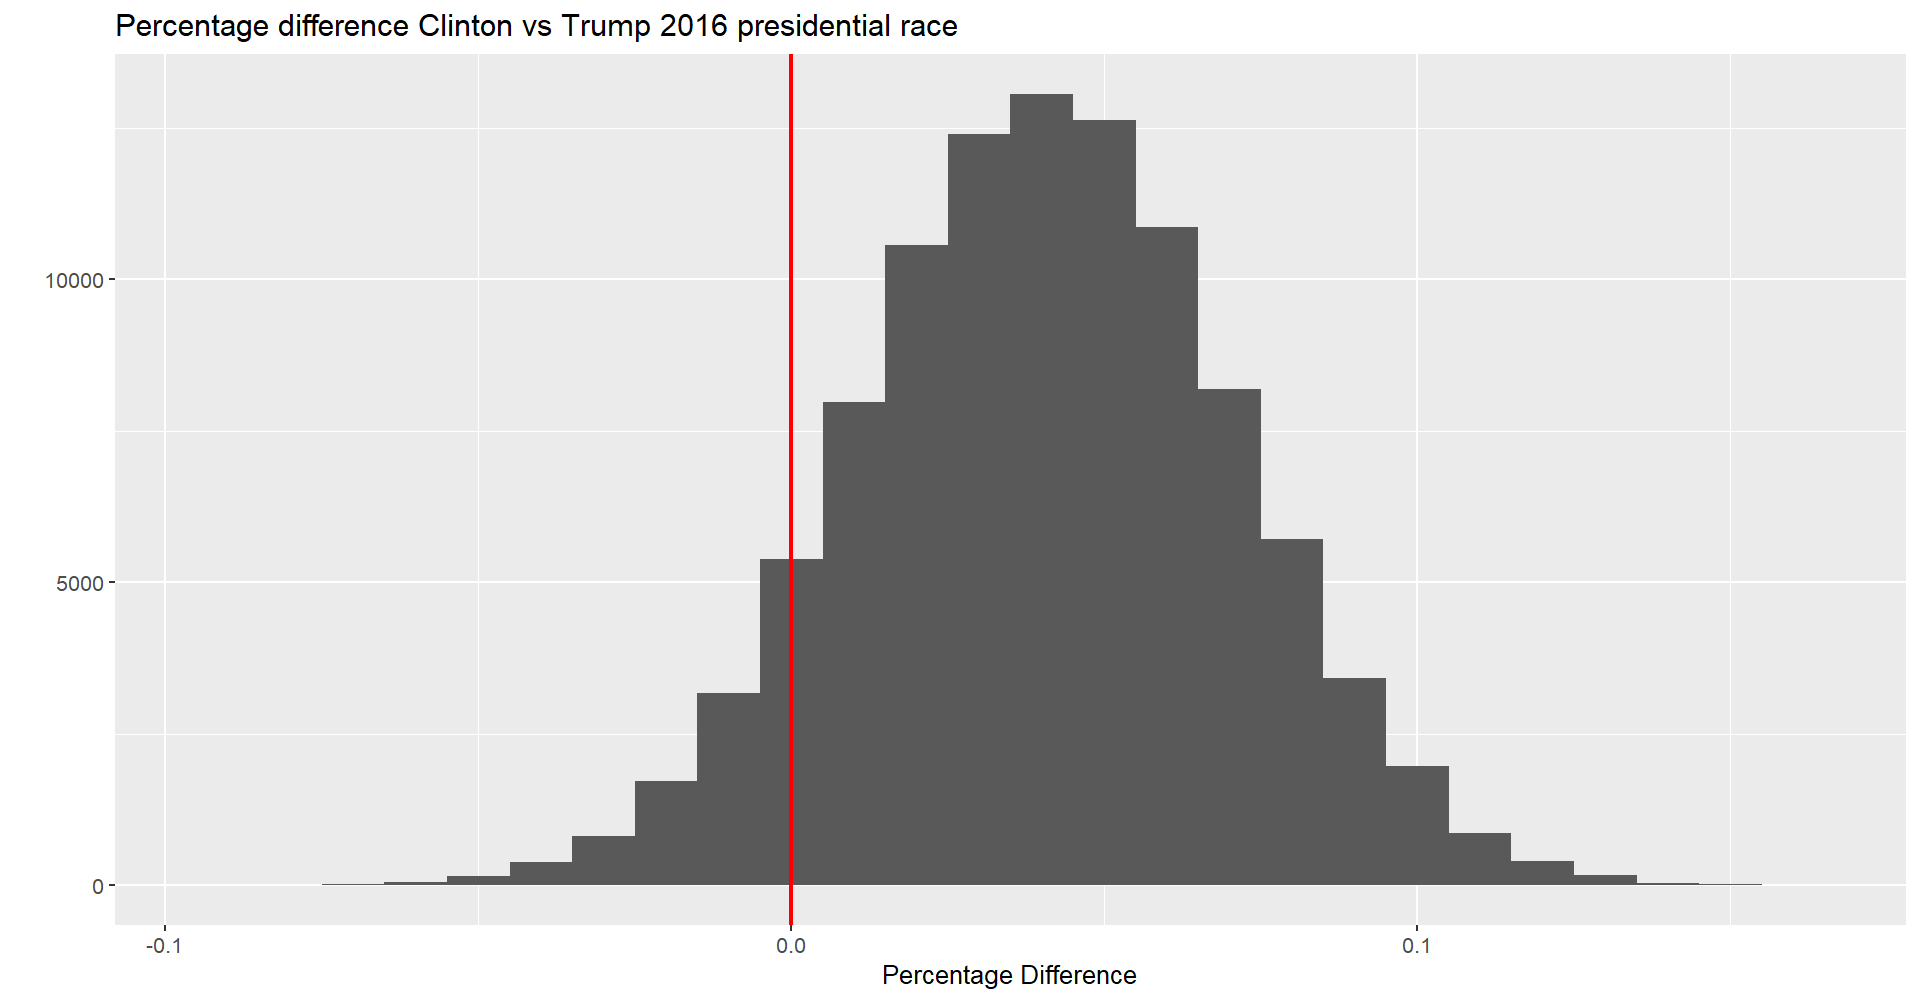
\includegraphics[width=340pt, height=200pt]{Chapters/chapter4/figures/hiillaryVStrump.png}
	%%\centerline{\epsfig{/Chapters/chapter1/figures/cat.eps,width=.8\textheight,height=.4\textwidth}}
	\caption[List of figure caption goes here]{Percentage difference: Hillary Clinton vs Donald Trump, five-way race.}\label{fig41}
\end{figure}

There is a 95\% probability that the percentage difference between Hillary and Trump according to this poll is (-1.8\%, 9.9\%). The probability of Hillary having more supporters is 91.3\%


\begin{tcolorbox}[enhanced,width=4.67in,center upper,
	fontupper=\large\bfseries,drop shadow southwest,sharp corners]
	\textit{R code. Multinomial-Dirichlet model: Polling 2016 USA presidential race}
\begin{VF}
\begin{lstlisting}[language=R]
# Predictive distribution by simulation
y0 <- c(44, 40, 16)
Pred <- apply(thetas, 1, function(p) {rmultinom(1, size = sum(y0), prob = p)})
sum(sapply(1:S, function(s) {sum(Pred[,s] == y0) == 3}))/S
0.00825
# Predictive distribution by analytical expression
PredY0 <- function(y0){
	n <- sum(y0)
	Res1 <- sum(sapply(1:length(y), function(l){lgamma(alphan[l]+y0[l]) - lgamma(alphan[l])-lfactorial(y0[l])}))
	Res <- lfactorial(n)+lgamma(sum(alphan))-lgamma(sum(alphan)+n) + Res1
	return(exp(Res))
}
PredY0(y0)
0.00850         
\end{lstlisting}
\end{VF}
\end{tcolorbox} 

The probability that from one hundred random selected people 44 support Hillary, 40 support Trump and 16 support other candidate is 0.85\%.

\item \textbf{Math test example continues}

You have a random sample of math scores of size $N=50$ from a normal distribution, $Y_i\sim \mathcal{N}(\mu, \sigma)$. The sample mean and variance are equal to $102$ and $10$, respectively. Using the normal-normal/inverse-gamma model where $\mu_0=100$, $\beta_0=1$, $\alpha_0=\delta_0=0.001$

\begin{itemize}
	\item Get 95\% confidence and credible intervals for $\mu$.
	\item What is the posterior probability that $\mu > 103$?  
\end{itemize}  

{\textbf{Answer}}

\begin{tcolorbox}[enhanced,width=4.67in,center upper,
	fontupper=\large\bfseries,drop shadow southwest,sharp corners]
	\textit{R code. Math test example continues}
\begin{VF}
\begin{lstlisting}[language=R]
set.seed(010101)
N <- 50
# Sample size
muhat <- 102
# Sample mean
sig2hat <- 10
# Sample variance
# Hyperparameters
mu0 <- 100
beta0 <- 1
delta0 <- 0.001
alpha0 <- 0.001
S <- 100000
# Posterior draws
alphan <- alpha0 + N
deltan <- sig2hat*(N - 1) + delta0 + beta0*N/(beta0 + N)*(muhat - mu0)^2
sig2Post <- invgamma::rinvgamma(S, shape = alphan, rate = deltan)
summary(sig2Post)
betan <- beta0 + N
mun <- (beta0*mu0 + N*muhat)/betan
muPost <- sapply(sig2Post, function(s2){rnorm(1, mun, sd = (s2/betan)^0.5)})
muPostq <- quantile(muPost, c(0.025, 0.5, 0.975))
muPostq
   2.5%      50%    97.5% 
101.0929 101.9625 102.8311
cutoff <- 103
PmuPostcutoff <- mean(muPost > cutoff)
PmuPostcutoff
0.00994
# Using Student's t
muPost_t <- ((deltan/(alphan*betan))^0.5)*rt(S, alphan) + mun
c1 <- rgb(173,216,230,max = 255, alpha = 50, names = "lt.blue")
c2 <- rgb(255,192,203, max = 255, alpha = 50, names = "lt.pink")
hist(muPost, main = "Histogram: Posterior mean", xlab = "Posterior mean", col = c2)
hist(muPost_t, main = "Histogram: Posterior mean", xlab = "Posterior mean", add = T, col = c1)
muPost_tq <- quantile(muPost_t, c(0.025, 0.5, 0.975))
muPost_tq
2.5%      50%    97.5% 
101.0837 101.9608 102.8435
PmuPost_tcutoff <- mean(muPost_t > cutoff)
PmuPost_tcutoff
0.01087
\end{lstlisting}
\end{VF}
\end{tcolorbox} 

We perform our calculations using the posterior conditional distribution, and the posterior marginal distribution. Both procedures give similar results as we can observe from Figure \ref{fig42}.

\begin{figure}[!h]
	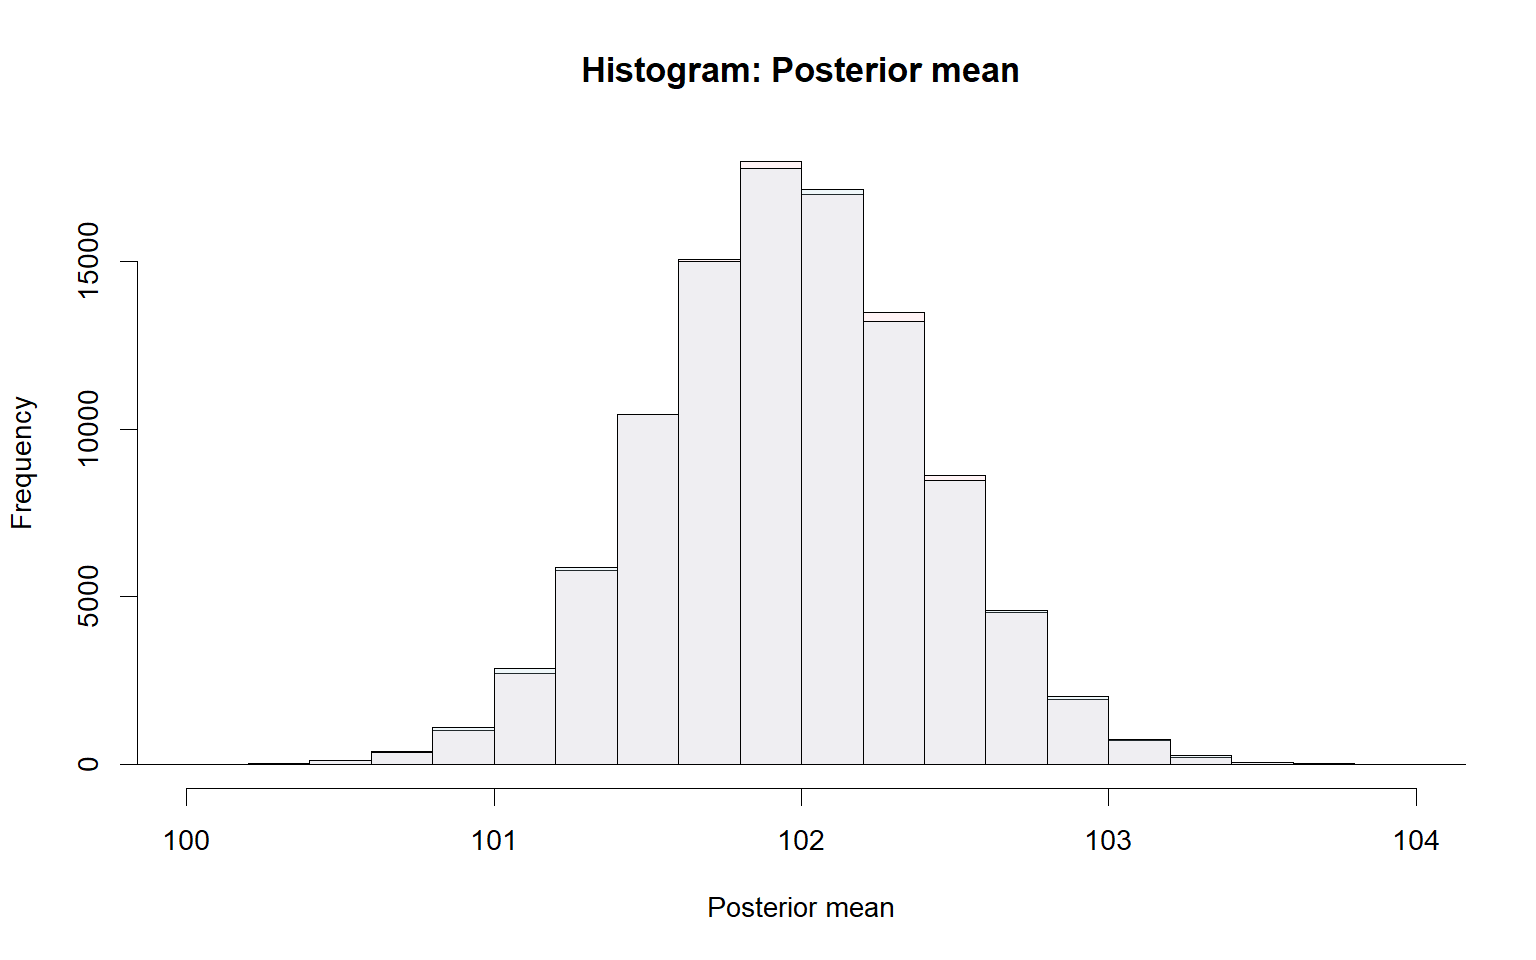
\includegraphics[width=340pt, height=200pt]{Chapters/chapter4/figures/conditionalVSmarginal.png}
	%%\centerline{\epsfig{/Chapters/chapter1/figures/cat.eps,width=.8\textheight,height=.4\textwidth}}
	\caption[List of figure caption goes here]{Histogram using the posterior conditional distribution and the posterior marginal distribution}\label{fig42}
\end{figure}


We have that the 95\% credible interval is (101.08, 102.84), and the probability of having a value greater than 103 is 1.09\%. 

%\item In the optimal tangency portfolio example, what are the equations for $\mu_{T+\kappa}=\mu_{n}$ and ${\bf\Sigma}_{T+\kappa}$? Use these equations to find the optimal weights six periods ahead using the tech stocks. 

%{\textbf{Answer}} 

\item \textbf{Demand of electricity example continues}

Set $c_0$ such that maximizes the marginal likelihood in the specifications with and without electricity price in the example of demand of electricity (empirical Bayes). Then, calculate the Bayes factor, and conclude if there is evidence supporting the inclusion of the price of electricity in the demand equation. 

{\textbf{Answer}} 

\begin{tcolorbox}[enhanced,width=4.67in,center upper,
	fontupper=\large\bfseries,drop shadow southwest,sharp corners]
	\textit{R code. Demand of electricity}
	\begin{VF}
		\begin{lstlisting}[language=R]
rm(list = ls())
set.seed(010101)
# Electricity demand
DataUt <- read.csv("https://raw.githubusercontent.com/besmarter/BSTApp/refs/heads/master/DataApp/Utilities.csv", sep = ",", header = TRUE, quote = "")
DataUtEst <- DataUt %>% 
filter(Electricity != 0)
attach(DataUtEst)
# Dependent variable: Monthly consumption (kWh) in log
Y <- log(Electricity)
N <- length(Y)
# Regressors quantity including intercept
X <- cbind(LnPriceElect, IndSocio1, IndSocio2, Altitude, Nrooms, HouseholdMem, Children, Lnincome, 1)
# Regressor without price
Xnew <- cbind(IndSocio1, IndSocio2, Altitude, Nrooms, HouseholdMem, Children, Lnincome, 1)
# Log marginal function (multiply by -1 due to minimization)
LogMarLikLM <- function(X, c0){
	k <- dim(X)[2]
	N <- dim(X)[1]	
	# Hyperparameters
	B0 <- c0*diag(k)
	b0 <- rep(0, k)
	# Posterior parameters
	bhat <- solve(t(X)%*%X)%*%t(X)%*%Y
	# Force this matrix to be symmetric
	Bn <- as.matrix(Matrix::forceSymmetric(solve(solve(B0) + t(X)%*%X))) 
	bn <- Bn%*%(solve(B0)%*%b0 + t(X)%*%X%*%bhat)
	dn <- as.numeric(d0 + t(Y)%*%Y+t(b0)%*%solve(B0)%*%b0-t(bn)%*%solve(Bn)%*%bn)
	an <- a0 + N
	# Log marginal likelihood
	logpy <- (N/2)*log(1/pi)+(a0/2)*log(d0)-(an/2)*log(dn) + 0.5*log(det(Bn)/det(B0)) + lgamma(an/2)-lgamma(a0/2)
	return(-logpy)
}
# Hyperparameters
d0 <- 0.001/2
a0 <- 0.001/2
# Empirical Bayes: Obtain c0 maximizing the log marginal likelihood
c0 <- 1000 
EB <- optim(c0, fn = LogMarLikLM, method = "Brent", lower = 0.0001, upper = 10^6, X = X)
EBnew <- optim(c0, fn = LogMarLikLM, method = "Brent", lower = 0.0001, upper = 10^6, X = Xnew)
# Change of order to take into account the -1 in the LogMarLikLM function
BFEM <- exp(EBnew$value - EB$value) 
BFEM
71897938
\end{lstlisting}
	\end{VF}
\end{tcolorbox} 

The Bayes factor based on the empirical Bayes of the model with electricity price versus the model without electricity price is equal to 71897938, this gives very strong evidence to include the price in the specification.
 
\item \textbf{Utility demand}

Use the file \textit{Utilities.csv} to estimate a multivariate linear regression model where $\mathbf{Y}_i=\left[\log(\text{electricity}_i) \ \log(\text{water}_i) \ \log(\text{gas}_i)\right]$ as function of $\log(\text{electricity price}_i)$, $\log(\text{water price}_i)$, $\log(\text{gas price}_i)$, $\text{IndSocio1}_i$, $\text{IndSocio2}_i$, $\text{Altitude}_i$, $\text{Nrooms}_i$, $\text{HouseholdMem}_i$, $\text{Children}_i$, and $\log(\text{Income}_i)$, where electricity, water and gas are monthly consumption of electricity (kWh), water (m$^3$) and gas (m$^3$), and other definitions are given in the Example of Section 4.3. Omit households that do not consume any of the utilities in this exercise. 

Set a non-informative prior framework, $\mathbf{B}_0=\left[0\right]_{11\times 3}$, $\mathbf{V}_0=1000 \mathbf{I}_{11}$, $\mathbf{\Psi}_0=1000 \mathbf{I}_{3}$ and $\alpha_0=3$, where we have $K=11$ (regressors plus intercept) and $M=3$ (equations) in this exercise.

\begin{enumerate}
	\item Find the posterior mean estimates and the highest posterior density intervals at 95\% of $\mathbf{B}$ and $\mathbf{\Sigma}$. Use the marginal distribution and the conditional distribution to obtain the posterior estimates of  $\mathbf{B}$, and compare the results.
	\item Find the Bayes factor comparing the baseline model in this exercise with the same specification but using the income in dollars. Now, calculate the Bayes factor using the income in thousand dollars. Is there any difference?
	\item Find the predictive distribution for the monthly demand of electricity, water and gas in the baseline specification of a household located in the lowest socioeconomic condition in a municipality located below 1000 meters above the sea level, 2 rooms, 3 members with children, a monthly income equal to USD 500, an electricity price equal to USD/kWh 0.15, a water price equal to USD/M$^3$ 0.70, and a gas price equal to USD/M$^3$ 0.75. 
\end{enumerate}   

{\textbf{Answer}} 

We see that the posterior estimates of the location parameters based on the marginal distribution and the conditional distribution are very similar (conditional on $\mathbf{\Sigma}$). This is important as many times there is no analytical solutions in well-known forms of marginal posterior distributions, and consequently, we should get draws of the posterior distributions based on conditional distributions of block of parameters (See Chapter \ref{chap5}).

We find that the Bayes factor of the baseline model ($\log(\text{Income})$) versus the two alternative models using income in dollars and thousand dollars are 108925764 and 0.1089261. The former gives strong evidence in favor of the baseline model, whereas the latter gives positive evidence for the model using the income in thousand dollars. This result despite that the location coefficients are the same in the two alternative specifications, except for the change in scale of the coefficients associated with income. This example shows that Bayes factors are sensitive to units of measure, and consequently, it is relevant to think carefully about the priors when performing hypothesis testing using a Bayesian framework. Observe that a nice feature in Bayesian inference is that we followed the same conceptual framework (Bayes factor) in the previous exercise and this exercise. In one hand, the previous exercise is an example of nested models, that is, one model is a restricted version of a more general model. On the other hand, this exercise is an example of non-nested models. This is not the case in the Frequentist approach. The statistical framework is not the same when testing nested and non-nested models.

\begin{tcolorbox}[enhanced,width=4.67in,center upper,
	fontupper=\large\bfseries,drop shadow southwest,sharp corners]
	\textit{R code. Utilities demand: Multivariate regression, posterior inference}
	\begin{VF}
		\begin{lstlisting}[language=R]
rm(list = ls())
set.seed(010101)
library(dplyr)
# Electricity demand
DataUt <- read.csv("https://raw.githubusercontent.com/besmarter/BSTApp/refs/heads/master/DataApp/Utilities.csv", sep = ",", header = TRUE, quote = "")
DataUtEst <- DataUt %>%  
filter(Electricity != 0 & Water !=0 & Gas != 0)
attach(DataUtEst)
Y <- cbind(log(Electricity), log(Water), log(Gas))
X <- cbind(LnPriceElect, LnPriceWater, LnPriceGas, IndSocio1, IndSocio2, Altitude, Nrooms, HouseholdMem, Children, Lnincome, 1)
M <- dim(Y)[2]
K <- dim(X)[2]
N <- dim(Y)[1]
# Hyperparameters
B0 <- matrix(0, K, M)
c0 <- 1000
V0 <- c0*diag(K)
Psi0 <- c0*diag(M)
a0 <- M
# Posterior parameters
Bhat <- solve(t(X)%*%X)%*%t(X)%*%Y 
S <- t(Y - X%*%Bhat)%*%(Y - X%*%Bhat)
Vn <- solve(solve(V0) + t(X)%*%X) 
Bn <- Vn%*%(solve(V0)%*%B0 + t(X)%*%X%*%Bhat)
Psin <- Psi0 + S + t(B0)%*%solve(V0)%*%B0 + t(Bhat)%*%t(X)%*%X%*%Bhat - t(Bn)%*%solve(Vn)%*%Bn
an <- a0 + N
#Posterior draws
s <- 10000 #Number of posterior draws
SIGs <- replicate(s, LaplacesDemon::rinvwishart(an, Psin))
BsCond <- sapply(1:s, function(s) {MixMatrix::rmatrixnorm(n = 1, mean=Bn, U = Vn,V = SIGs[,,s])})
summary(coda::mcmc(t(BsCond)))
Bs <- sapply(1:s, function(s) {MixMatrix::rmatrixt(n = 1, mean=Bn, U = Vn,V = Psin, df = an + 1 - M)})
summary(coda::mcmc(t(Bs)))
SIGMs <- t(sapply(1:s, function(l) {gdata::lowerTriangle(SIGs[,,l], diag=TRUE, byrow=FALSE)}))
summary(coda::mcmc(SIGMs))
hdiBs <- HDInterval::hdi(t(BsCond), credMass = 0.95) # Highest posterior density credible interval
hdiBs
hdiSIG <- HDInterval::hdi(SIGMs, credMass = 0.95) # Highest posterior density credible interval
hdiSIG
		\end{lstlisting}
	\end{VF}
\end{tcolorbox} 

\begin{tcolorbox}[enhanced,width=4.67in,center upper,
	fontupper=\large\bfseries,drop shadow southwest,sharp corners]
	\textit{R code. Utilities demand: Multivariate regression, Bayes factors}
	\begin{VF}
		\begin{lstlisting}[language=R]
# Log marginal function (multiply by -1 due to minimization)
LogMarLikLM <- function(X, c0){
	c10 <- c0[1]; c20 <- c0[2]
	k <- dim(X)[2]
	N <- dim(X)[1]
	# Hyperparameters
	V0 <- c10*diag(K)
	Psi0 <- c20*diag(M)
	# Posterior parameters
	Bhat <- solve(t(X)%*%X)%*%t(X)%*%Y 
	S <- t(Y - X%*%Bhat)%*%(Y - X%*%Bhat)
	Vn <- solve(solve(V0) + t(X)%*%X) 
	Bn <- Vn%*%(solve(V0)%*%B0 + t(X)%*%X%*%Bhat)
	Psin <- Psi0 + S + t(B0)%*%solve(V0)%*%B0 + t(Bhat)%*%t(X)%*%X%*%Bhat - t(Bn)%*%solve(Vn)%*%Bn
	# Log marginal likelihood
	logpy <- (N*M/2)*log(1/pi)+(a0/2)*log(det(Psi0)) - (an/2)*log(det(Psin)) + (M/2)*(log(det(Vn)) - log(det(V0))) + lgamma(an/2)-lgamma(a0/2)
	return(-logpy)
}
c0 <- rep(1000, 2)
LogML <- LogMarLikLM(X=X, c0 = c0)
# Using income in dollars as regressor
Xnew <- cbind(LnPriceElect, LnPriceWater, LnPriceGas, IndSocio1, IndSocio2, Altitude, Nrooms, HouseholdMem, Children, exp(Lnincome), 1)
LogMLnew <- LogMarLikLM(X=Xnew, c0 = c0)
# Bayes factor
BF12 <- exp(LogMLnew - LogML)
BF12
# Using income in thousand dollars as regressor
XnewT <- cbind(LnPriceElect, LnPriceWater, LnPriceGas, IndSocio1, IndSocio2, Altitude, Nrooms, HouseholdMem, Children, exp(Lnincome)/1000, 1)
LogMLnewT <- LogMarLikLM(X=XnewT, c0 = c0)
# Bayes factor
BF13 <- exp(LogMLnewT - LogML)
BF13
		\end{lstlisting}
	\end{VF}
\end{tcolorbox} 

\begin{tcolorbox}[enhanced,width=4.67in,center upper,
	fontupper=\large\bfseries,drop shadow southwest,sharp corners]
	\textit{R code. Utilities demand: Multivariate regression, predictive distribution}
	\begin{VF}
		\begin{lstlisting}[language=R]
# Predictive distribution
Xpred <- c(log(0.15), log(0.70), log(0.75), 1, 0, 0, 2, 3, 1, log(500), 1)
Mean <- Xpred%*%Bn
Hn <- 1+t(Xpred)%*%Vn%*%Xpred
UtilDemand <- exp(replicate(s, MixMatrix::rmatrixt(n = 1, mean=Mean, U = Hn, V = Psin, df = an + 1 - M)))
ElePred <- UtilDemand[1,1,]
WatPred <- UtilDemand[1,2,]
GasPred <- UtilDemand[1,3,]
data <- data.frame(cbind(ElePred, WatPred, GasPred)) #Data frame
annotations1 <- data.frame(
x = round(quantile(data$ElePred, c(0.025, 0.5, 0.975)),1),
y = c(600, 1000, 600),
label = c("2.5%:", "50%:", "97.5%:")
)
annotations2 <- data.frame(
x = round(quantile(data$WatPred, c(0.025, 0.5, 0.975)),1),
y = c(600, 1000, 600),
label = c("2.5%:", "50%:", "97.5%:")
)
annotations3 <- data.frame(
x = round(quantile(data$GasPred, c(0.025, 0.5, 0.975)),1),
y = c(600, 1000, 600),
label = c("2.5%:", "50%:", "97.5%:")
)
require(ggplot2) # Cool figures
require(ggpubr) # Multiple figures in one page
require(latex2exp) # LaTeX equations in figures
fig1 <- ggplot(data = data, aes(ElePred)) + geom_histogram(bins = 40, color = "#000000", fill = "#0099F8") + 	xlab("kWh") + ylab("Frequency") +	ggtitle("Electricity") + xlim(0, 1050) + geom_text(data = annotations1, aes(x = x, y = y, label = paste(label, x)), size = 3, fontface = "bold")
fig2 <- ggplot(data = data, aes(WatPred)) + geom_histogram(bins = 40, color = "#000000", fill = "#0099F8") + 	xlab(TeX("$M^3$")) + ylab("Frequency") +	ggtitle("Water") + xlim(0, 100) + geom_text(data = annotations2, aes(x = x, y = y, label = paste(label, x)), size = 3, fontface = "bold")
fig3 <- ggplot(data = data, aes(GasPred)) + geom_histogram(bins = 40, color = "#000000", fill = "#0099F8") + 	xlab(TeX("$M^3$")) + ylab("Frequency") +	ggtitle("Gas") + xlim(0, 80) + geom_text(data = annotations3, aes(x = x, y = y, label = paste(label, x)), size = 3, fontface = "bold")
		\end{lstlisting}
	\end{VF}
\end{tcolorbox} 


Figures \ref{fig13}, \ref{fig14} and \ref{fig15} show the marginal predictive distributions of electricity, water and gas for the reference household. The median predictive values are kWh 168.8, M$^3$ 12.3 and M$^3$ 10.1, respectively. In addition, the 95\% credible intervals are (27.7, 1028.9), (1.5, 98.7) and (1.5, 67.5) for electricity, water and gas.  

\begin{figure}[!h]
	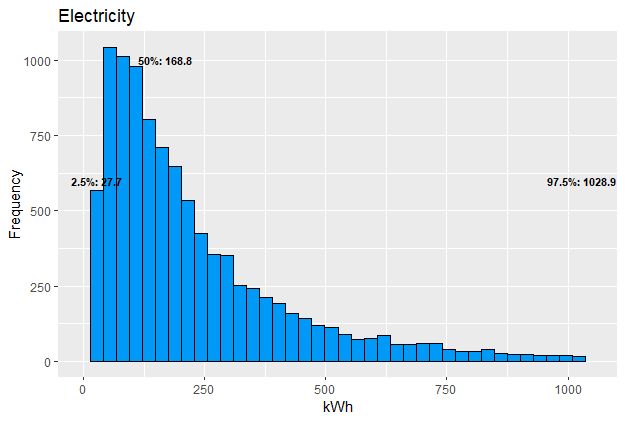
\includegraphics[width=340pt, height=200pt]{Chapters/chapter4/figures/ElectMulti.png}
	%%\centerline{\epsfig{/Chapters/chapter1/figures/cat.eps,width=.8\textheight,height=.4\textwidth}}
	\caption[List of figure caption goes here]{Histogram using the posterior predictive distribution of electricity demand}\label{fig13}
\end{figure}

\begin{figure}[!h]
	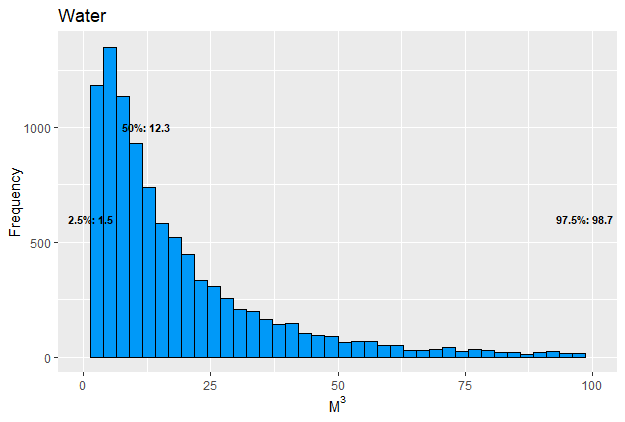
\includegraphics[width=340pt, height=200pt]{Chapters/chapter4/figures/WaterMulti.png}
	%%\centerline{\epsfig{/Chapters/chapter1/figures/cat.eps,width=.8\textheight,height=.4\textwidth}}
	\caption[List of figure caption goes here]{Histogram using the posterior predictive distribution of water demand}\label{fig14}
\end{figure}  

\begin{figure}[!h]
	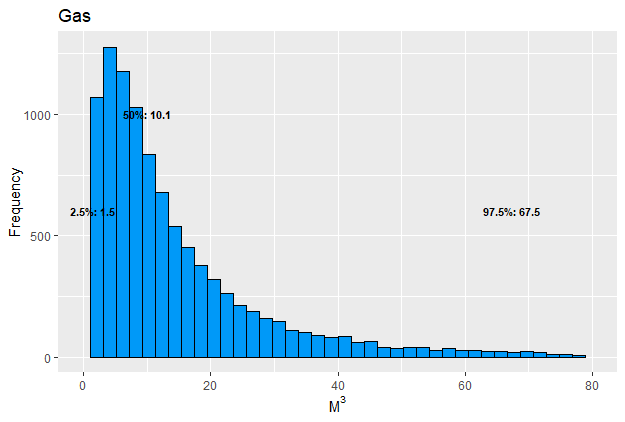
\includegraphics[width=340pt, height=200pt]{Chapters/chapter4/figures/GasMulti.png}
	%%\centerline{\epsfig{/Chapters/chapter1/figures/cat.eps,width=.8\textheight,height=.4\textwidth}}
	\caption[List of figure caption goes here]{Histogram using the posterior predictive distribution of gas demand}\label{fig15}
\end{figure}    
\end{enumerate}





\bibliographystyle{plain}
\bibliography{bibtex_example}

\printindex

\end{document}
